%%%%%%%%%%%%%%%%%%%%%%%%%%%%%%%%%%%%%%%%%%%%%%%%%%%%%%%%%%%%%%%%%%%%%%%%%%%%
% AGUtmpl.tex: this template file is for articles formatted with LaTeX2e,
% Modified December 2018
%
% This template includes commands and instructions
% given in the order necessary to produce a final output that will
% satisfy AGU requirements.
%
% FOR FIGURES, DO NOT USE \psfrag
%
%%%%%%%%%%%%%%%%%%%%%%%%%%%%%%%%%%%%%%%%%%%%%%%%%%%%%%%%%%%%%%%%%%%%%%%%%%%%
%
% IMPORTANT NOTE:
%
% SUPPORTING INFORMATION DOCUMENTATION IS NOT COPYEDITED BEFORE PUBLICATION.
%
%
%
%%%%%%%%%%%%%%%%%%%%%%%%%%%%%%%%%%%%%%%%%%%%%%%%%%%%%%%%%%%%%%%%%%%%%%%%%%%%
%
% Step 1: Set the \documentclass
%
%
% PLEASE USE THE DRAFT OPTION TO SUBMIT YOUR PAPERS.
% The draft option produces double spaced output.
%
% Choose the journal abbreviation for the journal you are
% submitting to:

% jgrga JOURNAL OF GEOPHYSICAL RESEARCH (use for all of them)
% gbc   GLOBAL BIOCHEMICAL CYCLES
% grl   GEOPHYSICAL RESEARCH LETTERS
% pal   PALEOCEANOGRAPHY
% ras   RADIO SCIENCE
% rog   REVIEWS OF GEOPHYSICS
% tec   TECTONICS
% wrr   WATER RESOURCES RESEARCH
% gc    GEOCHEMISTRY, GEOPHYSICS, GEOSYSTEMS
% sw    SPACE WEATHER
% ms    JAMES
% ef    EARTH'S FUTURE
%
%
%
% (If you are submitting to a journal other than jgrga,
% substitute the initials of the journal for "jgrga" below.)

\documentclass[draft,jgrga]{agutexSI2019}

%%%%%%%%%%%%%%%%%%%%%%%%%%%%%%%%%%%%%%%%%%%%%%%%%%%%%%%%%%%%%%%%%%%%%%%%%
%
%  SUPPORTING INFORMATION TEMPLATE
%
%% ------------------------------------------------------------------------ %%
%
%
%Please use this template when formatting and submitting your Supporting Information.

%This template serves as both a “table of contents” for the supporting information for your article and as a summary of files.
%
%
%OVERVIEW
%
%Please note that all supporting information will be peer reviewed with your manuscript. It will not be copyedited if the paper is accepted.
%In general, the purpose of the supporting information is to enable authors to provide and archive auxiliary information such as data tables, method information, figures, video, or computer software, in digital formats so that other scientists can use it.
%The key criteria are that the data:
% 1. supplement the main scientific conclusions of the paper but are not essential to the conclusions (with the exception of
%    including %data so the experiment can be reproducible);
% 2. are likely to be usable or used by other scientists working in the field;
% 3. are described with sufficient precision that other scientists can understand them, and
% 4. are not exe files.
%
%USING THIS TEMPLATE
%
%***All references should be included in the reference list of the main paper so that they can be indexed, linked, and counted as citations.  The reference section does not count toward length limits.
%
%All Supporting text and figures should be included in this document. Insert supporting information content into each appropriate section of the template. To add additional captions, simply copy and paste each sample as needed.

%Tables may be included, but can also be uploaded separately, especially if they are larger than 1 page, or if necessary for retaining table formatting. Data sets, large tables, movie files, and audio files should be uploaded separately. Include their captions in this document and list the file name with the caption. You will be prompted to upload these files on the Upload Files tab during the submission process, using file type “Supporting Information (SI)”

%IMPORTANT NOTE ON FIGURES AND TABLES
% Placeholders for figures and tables appear after the \end{article} command, after references.
% DO NOT USE \psfrag or \subfigure commands.
%
 \usepackage{graphicx}
%
%  Uncomment the following command to allow illustrations to print
%   when using Draft:
 \setkeys{Gin}{draft=false}
%
% You may need to use one of these options for graphicx depending on the driver program you are using. 
%
% [xdvi], [dvipdf], [dvipsone], [dviwindo], [emtex], [dviwin],
% [pctexps],  [pctexwin],  [pctexhp],  [pctex32], [truetex], [tcidvi],
% [oztex], [textures]
%
%
%% ------------------------------------------------------------------------ %%
%
%  ENTER PREAMBLE
%
%% ------------------------------------------------------------------------ %%

% Author names in capital letters:
%\authorrunninghead{BALES ET AL.}

% Shorter version of title entered in capital letters:
%\titlerunninghead{SHORT TITLE}

%Corresponding author mailing address and e-mail address:
%\authoraddr{Corresponding author: A. B. Smith,
%Department of Hydrology and Water Resources, University of
%Arizona, Harshbarger Building 11, Tucson, AZ 85721, USA.
%(a.b.smith@hwr.arizona.edu)}
\newcommand{\markred}[1]{\textcolor{red}{#1}}
%\newcommand{\markcyan}[1]{\textcolor{cyan}{#1}}
\newcommand{\markblue}[1]{\textcolor{blue}{#1}}
%\newcommand{\markgreen}[1]{\textcolor{magenta}{#1}}


\begin{document}

%% ------------------------------------------------------------------------ %%
%
%  TITLE
%
%% ------------------------------------------------------------------------ %%

%\includegraphics{agu_pubart-white_reduced.eps}


\title{Supporting Information for "Local lydraulic conductivity in heterogeneous porous media"}
%
% e.g., \title{Supporting Information for "Terrestrial ring current:
% Origin, formation, and decay $\alpha\beta\Gamma\Delta$"}
%
%DOI: 10.1002/%insert paper number here%

%% ------------------------------------------------------------------------ %%
%
%  AUTHORS AND AFFILIATIONS
%
%% ------------------------------------------------------------------------ %%


% List authors by first name or initial followed by last name and
% separated by commas. Use \affil{} to number affiliations, and
% \thanks{} for author notes.
% Additional author notes should be indicated with \thanks{} (for
% example, for current addresses).

% Example: \authors{A. B. Author\affil{1}\thanks{Current address, Antartica}, B. C. Author\affil{2,3}, and D. E.
% Author\affil{3,4}\thanks{Also funded by Monsanto.}}


\authors{Quirine Krol \affil{1}, Itzhak Fouxon \affil{1,2}, Pascal Corso \affil{1}, Markus Holzner \affil{1,3,4}}



% \affiliation{1}{First Affiliation}
% \affiliation{2}{Second Affiliation}
% \affiliation{3}{Third Affiliation}
% \affiliation{4}{Fourth Affiliation}

\affiliation{1}{ETH Zurich, Stefano Franscini-Platz 5, 8093 Zurich, Switzerland}
\affiliation{2}{Department of Computational Science and Engineering, Yonsei University, Seoul 120-749, South Korea}
\affiliation{3}{Swiss Federal Institute for Water Science and Technology EAWAG}
\affiliation{4}{Swiss Federal Institute for Forest, Snow and Landscape Research WSL}
%(repeat as many times as is necessary)





%% ------------------------------------------------------------------------ %%
%
%  BEGIN ARTICLE
%
%% ------------------------------------------------------------------------ %%

% The body of the article must start with a \begin{article} command
%
% \end{article} must follow the references section, before the figures
%  and tables.

\begin{article}

%% ------------------------------------------------------------------------ %%
%
%  TEXT
%
%% ------------------------------------------------------------------------ %%



\noindent\textbf{Contents of this file}
%%%Remove or add items as needed%%%
\begin{enumerate}
\item Direct numerical simulation of Stokes flow in porous media and extaction of pore attributes.
\item Fitting models, results and model performance.
\item Measuring the Transversal and Longitunidinal Energy Dissipation tensor.
\item Histograms of $L_{\rm{eff}}$ and resistances $\mathcal{R}$.
%if Tables are larger than 1 page, upload as separate excel file
\end{enumerate}
\noindent\textbf{Additional Supporting Information (Files uploaded separately)}
\begin{enumerate}
\item Iso-pressure surfaces video
\item Pore identification video
\end{enumerate}

\section*{Introduction}
%Type or paste your text here. The introduction gives a brief overview of the supporting information. You should include information %about as many of the following as possible (when appropriate):
% 1. a general overview of the kind of data files;
% 2. information about when and how the data were collected or created;
% 3. a general description of processing steps used;
% 4. any known imperfections or anomalies in the data.

%\clearpage

%Delete all unused file types below. Copy/paste for multiples of each file type as needed.
Below we describe the necessary steps and specific settings of the analysis presented in methodology. The fist part consists of the description of the direct numerical simulations performed that are used as a numerical experiment, followed by details of the extraction of iso pressure surfaces and and their attributes necessary to calculate the pore resistance. The second part gives the details involving models, including a detailed overview of their performance. In the third section we show with an example that Eq.(6) is a reasonable assumption. In the last section we show the distributions of the local resistances and the integrated pore lengths and a very short description of a roadmap describing a possible application of a network model approach. 


\section{Direct numerical Simulations and extraction of pore attributes}

\subsection{Geometry of the porous media interface}
For all 3 media we have used a levelset of a Gaussian Random Field given by a spectral density as given in \cite{roberts_transport_1995}. Gaussian Random Fields are increasingly used for modeling porous media \cite{liu_advances_2019}. The porous media boundary is given by a level-set and was chosen such that we have porosity values of $0.68,0.34$ and $0.16$, for porous media 1, 2 and 3 respectively. The geometries are represented by 3 stl files that serve as input for the build-in meshing algorithm of Openfoam v. 4.1 \citeA{weller_tensorial_1998}. The bounding box of the porous media (inlet, outlet, upper and lower wall, front and back) are obtained with a BlockMesh. The meshing of the pore space is obtained with SnappyHexMesh with refinement levels 2, for a minimum and 3 for a maximum at the porous media boundary. The number of cells are $35,~ 31,\rm{and }~15$ Million respectively.

We inlcuded Table \ref{tab:results_geometries} that show a few geometrical parameters characterizing the porous media. The averaged pore size is defined by $l_p = 4 \phi/s$ with $s= |\Gamma|/V$ the specific surface area given by the ratio of porous media interface total area $|\Gamma|$ and the total volume $V$. The relative pore size $\ell_p/L$, with $L$ the porous media extend.  The surface roughness is defined by the standard deviation of the mean curvature $H$ divided by the average pore size $l_p$. These measures are introduced to show the wide range of chosen geometries. For example the roughness is smaller for the first porous media compared to the other two. This might indicate that the circularity of the iso-pressure surfaces will be higher, and will have a larger impact on the local hydraulic resistance.  

\vspace{1cm}
\begin{tabular}{l|c|c|c|c|c|c|c|c|c|c}\label{tab:results_geometries}
- & porosity & $s$ & $ l_p/L$ &  $\rm{std}(H)^{-1}/l_p$ \\
\hline
PM1 &$0.68$ & $2.0\times10^{4}$ & $0.17$ &  $0.14$ \\
PM2 & $0.34$ & $1.8\times10^{4}$ & $0.08$ &  $0.44$ \\
PM3 & $0.17$ & $1.2\times10^{4}$ & $0.06$ &  $0.35$ 
\end{tabular}

\subsection{Direct Numerical Simulations}

The flow in the three porous medium configurations was simulated using the open-source OpenFOAM software .
The three-dimensional meshes consisting in the majority of hexahedral cells were generated from the surface of the porous media represented as a tessellation of triangles. The meshes were obtained using the build-in SnappyHexMesh utility. For the three configurations, the meshes consist of approximately 10 million cells and the non-orthogonality between the faces of each cell is limited to 60°and the skewness (as defined within OpenFOAM) of the cells is at most equal to 4 \cite{moukalled_finite_2016}. The steady-state Navier-Stokes equations are resolved using the SIMPLE algorithm for coupling the pressure and momentum equations \cite{jasak_error_1996}. Relaxation factors were chosen to be equal to 0.7 for the momentum equation and 0.2 for the pressure equation in order to ensure stability. The choice of the spatial discretization schemes is made such that the simulations are second-order accurate. For the diffusive term, which is dominating for the range of Reynolds numbers considered in these simulations, a limiter for the computation of gradient at the interface between two cells is introduced to take into account the effect of cell non-orthogonality and skewness and at the same time to keep the solution bounded. 

Concerning boundary conditions, the velocity at the pore surface is set to zero. A pressure difference of 1 Pa at the two extremities perpendicular to the stream-wise direction of the box defining the computational domain is imposed. The dimension of the box in this direction is 1 mm. The lateral faces of the computational box are also associated with a zero-velocity condition. 
The simulations are initialized with PotentialFoam and run with SimpleFoam with standard residual controls of $10^{-6}$ for both the pressure and velocity fields. The Kinematic viscosity is set to $10^{-6}\rm{m^2s^{-1}}$, which is close to the value for water. The SimpleFoam solver took approximately 20, 8 and 3 hours to obtain the results using 32 cores. A visualization of the results for the three porous media is shown in Fig.2 of the main manuscript.

\begin{figure}[htbp!]
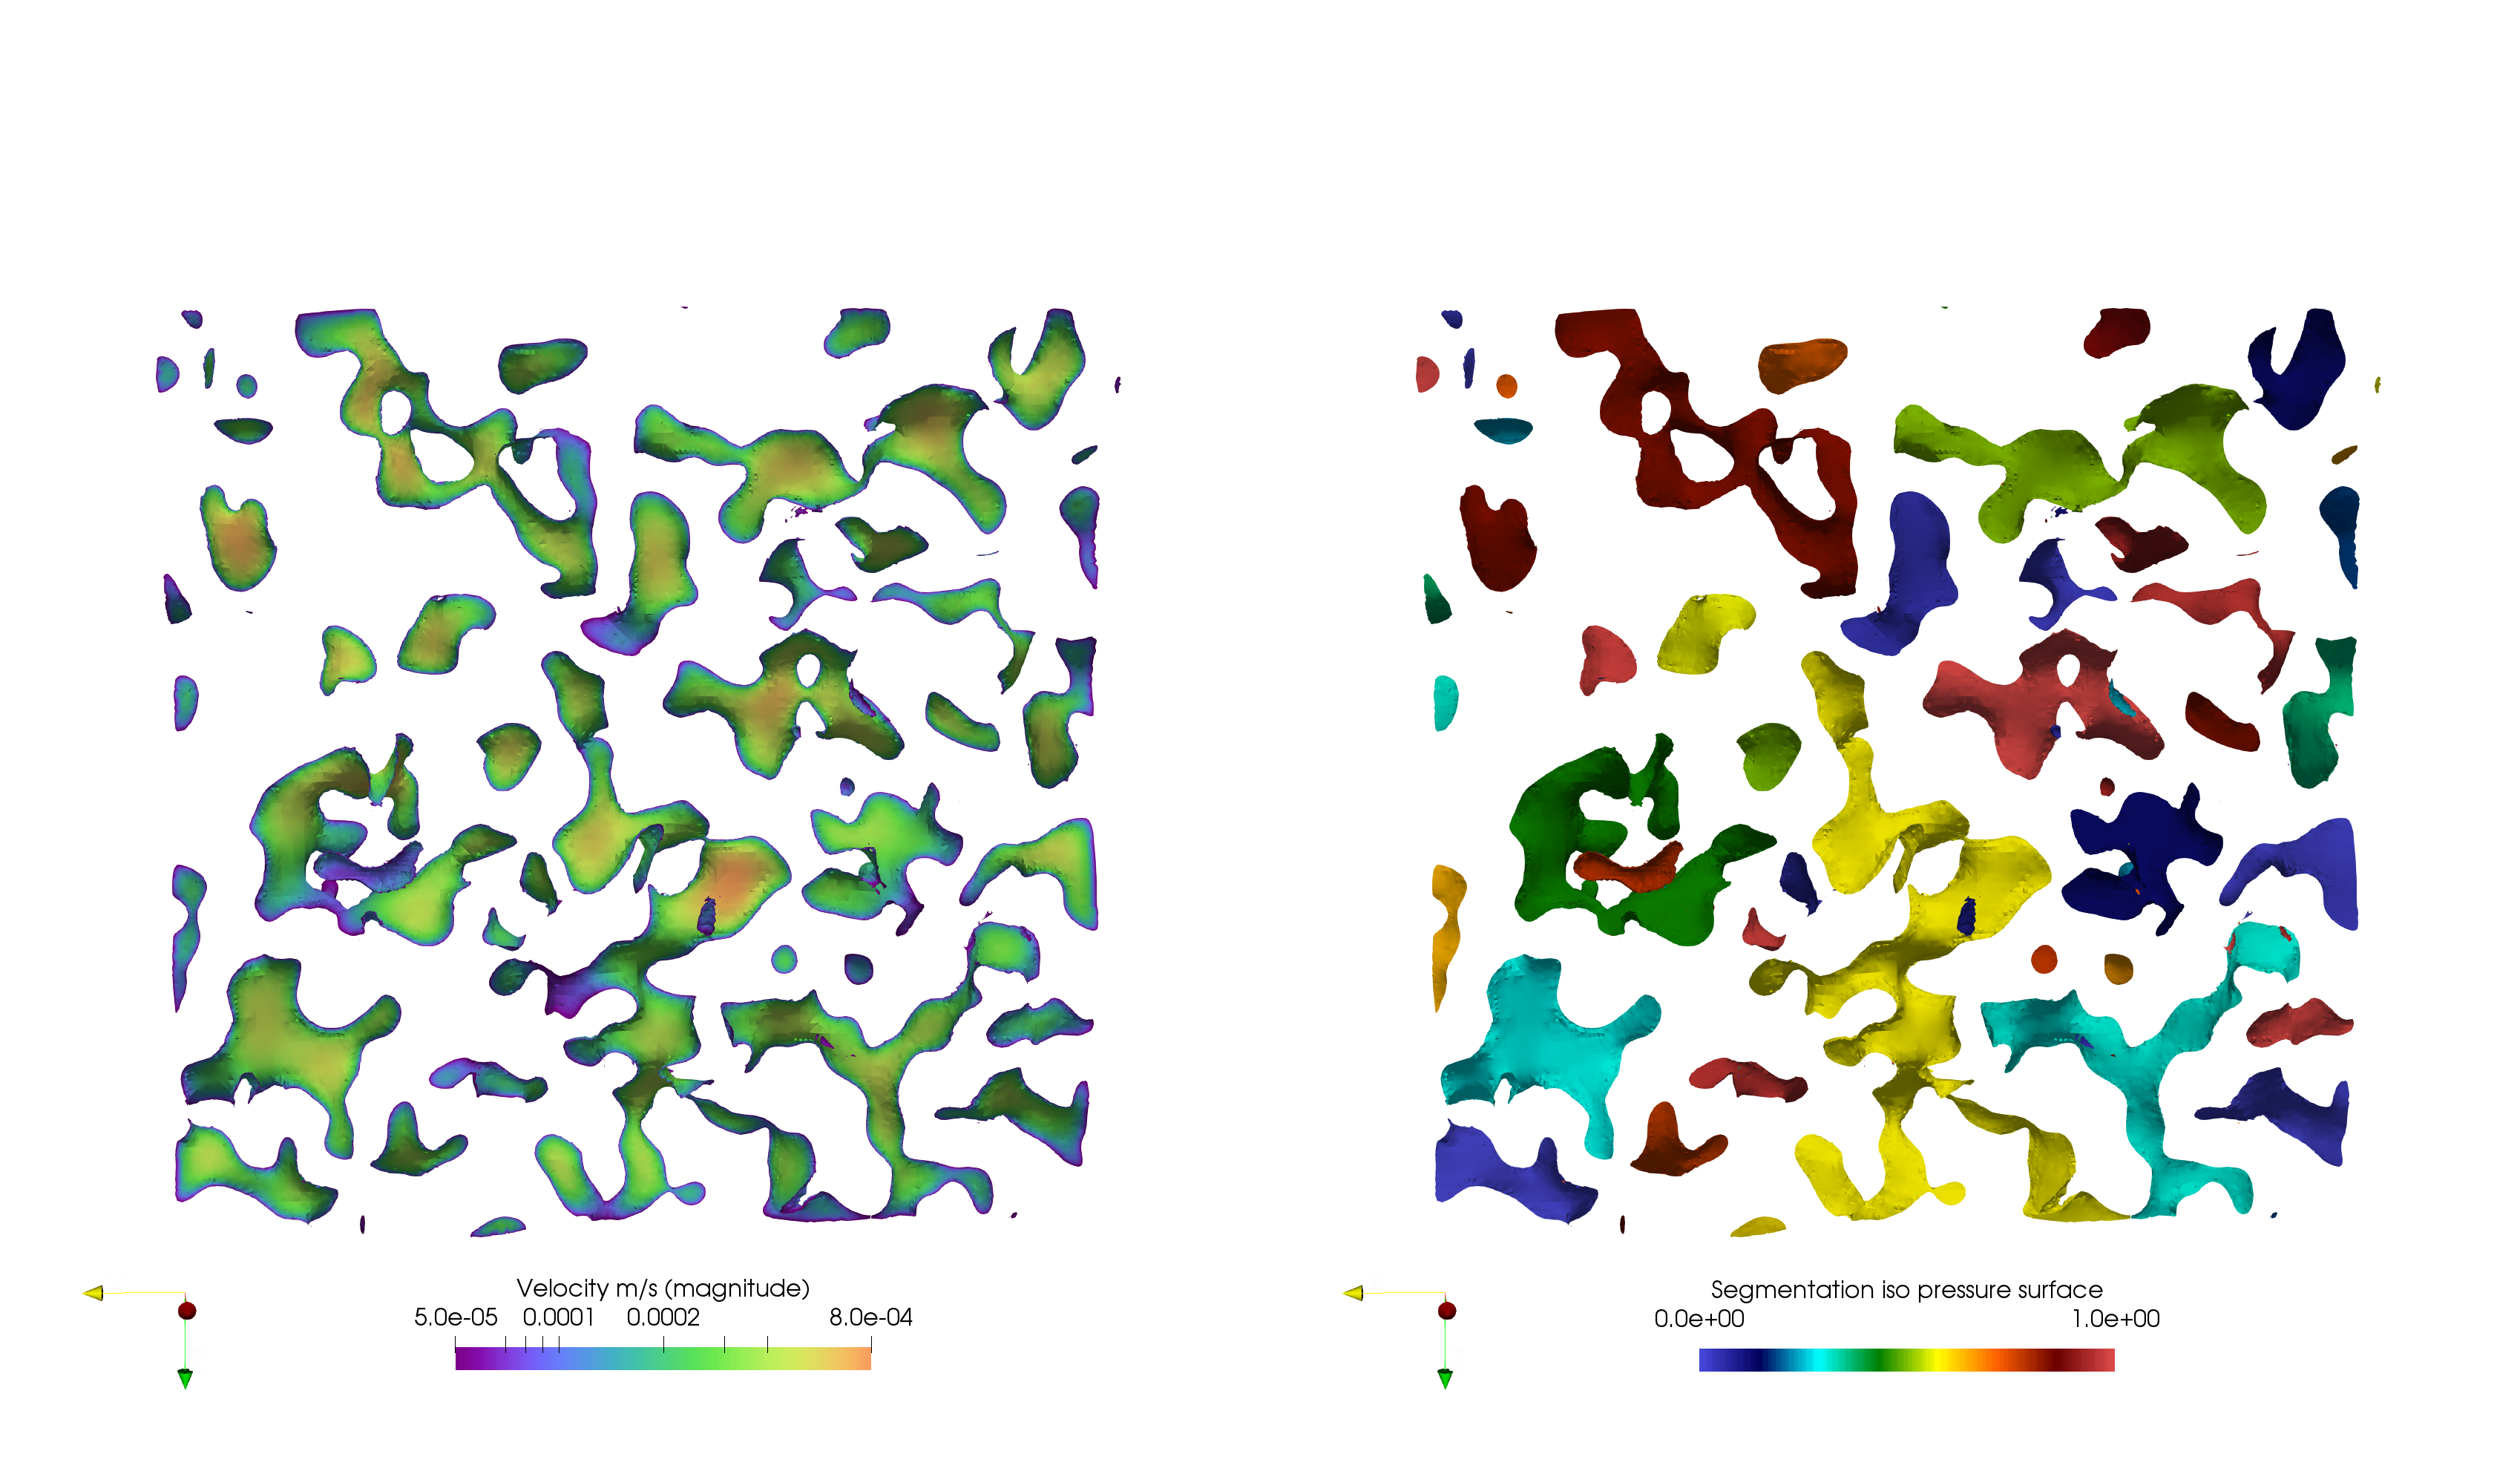
\includegraphics[height=6cm]{figures/semgentation_veloctiy_iso_p_surface.png}
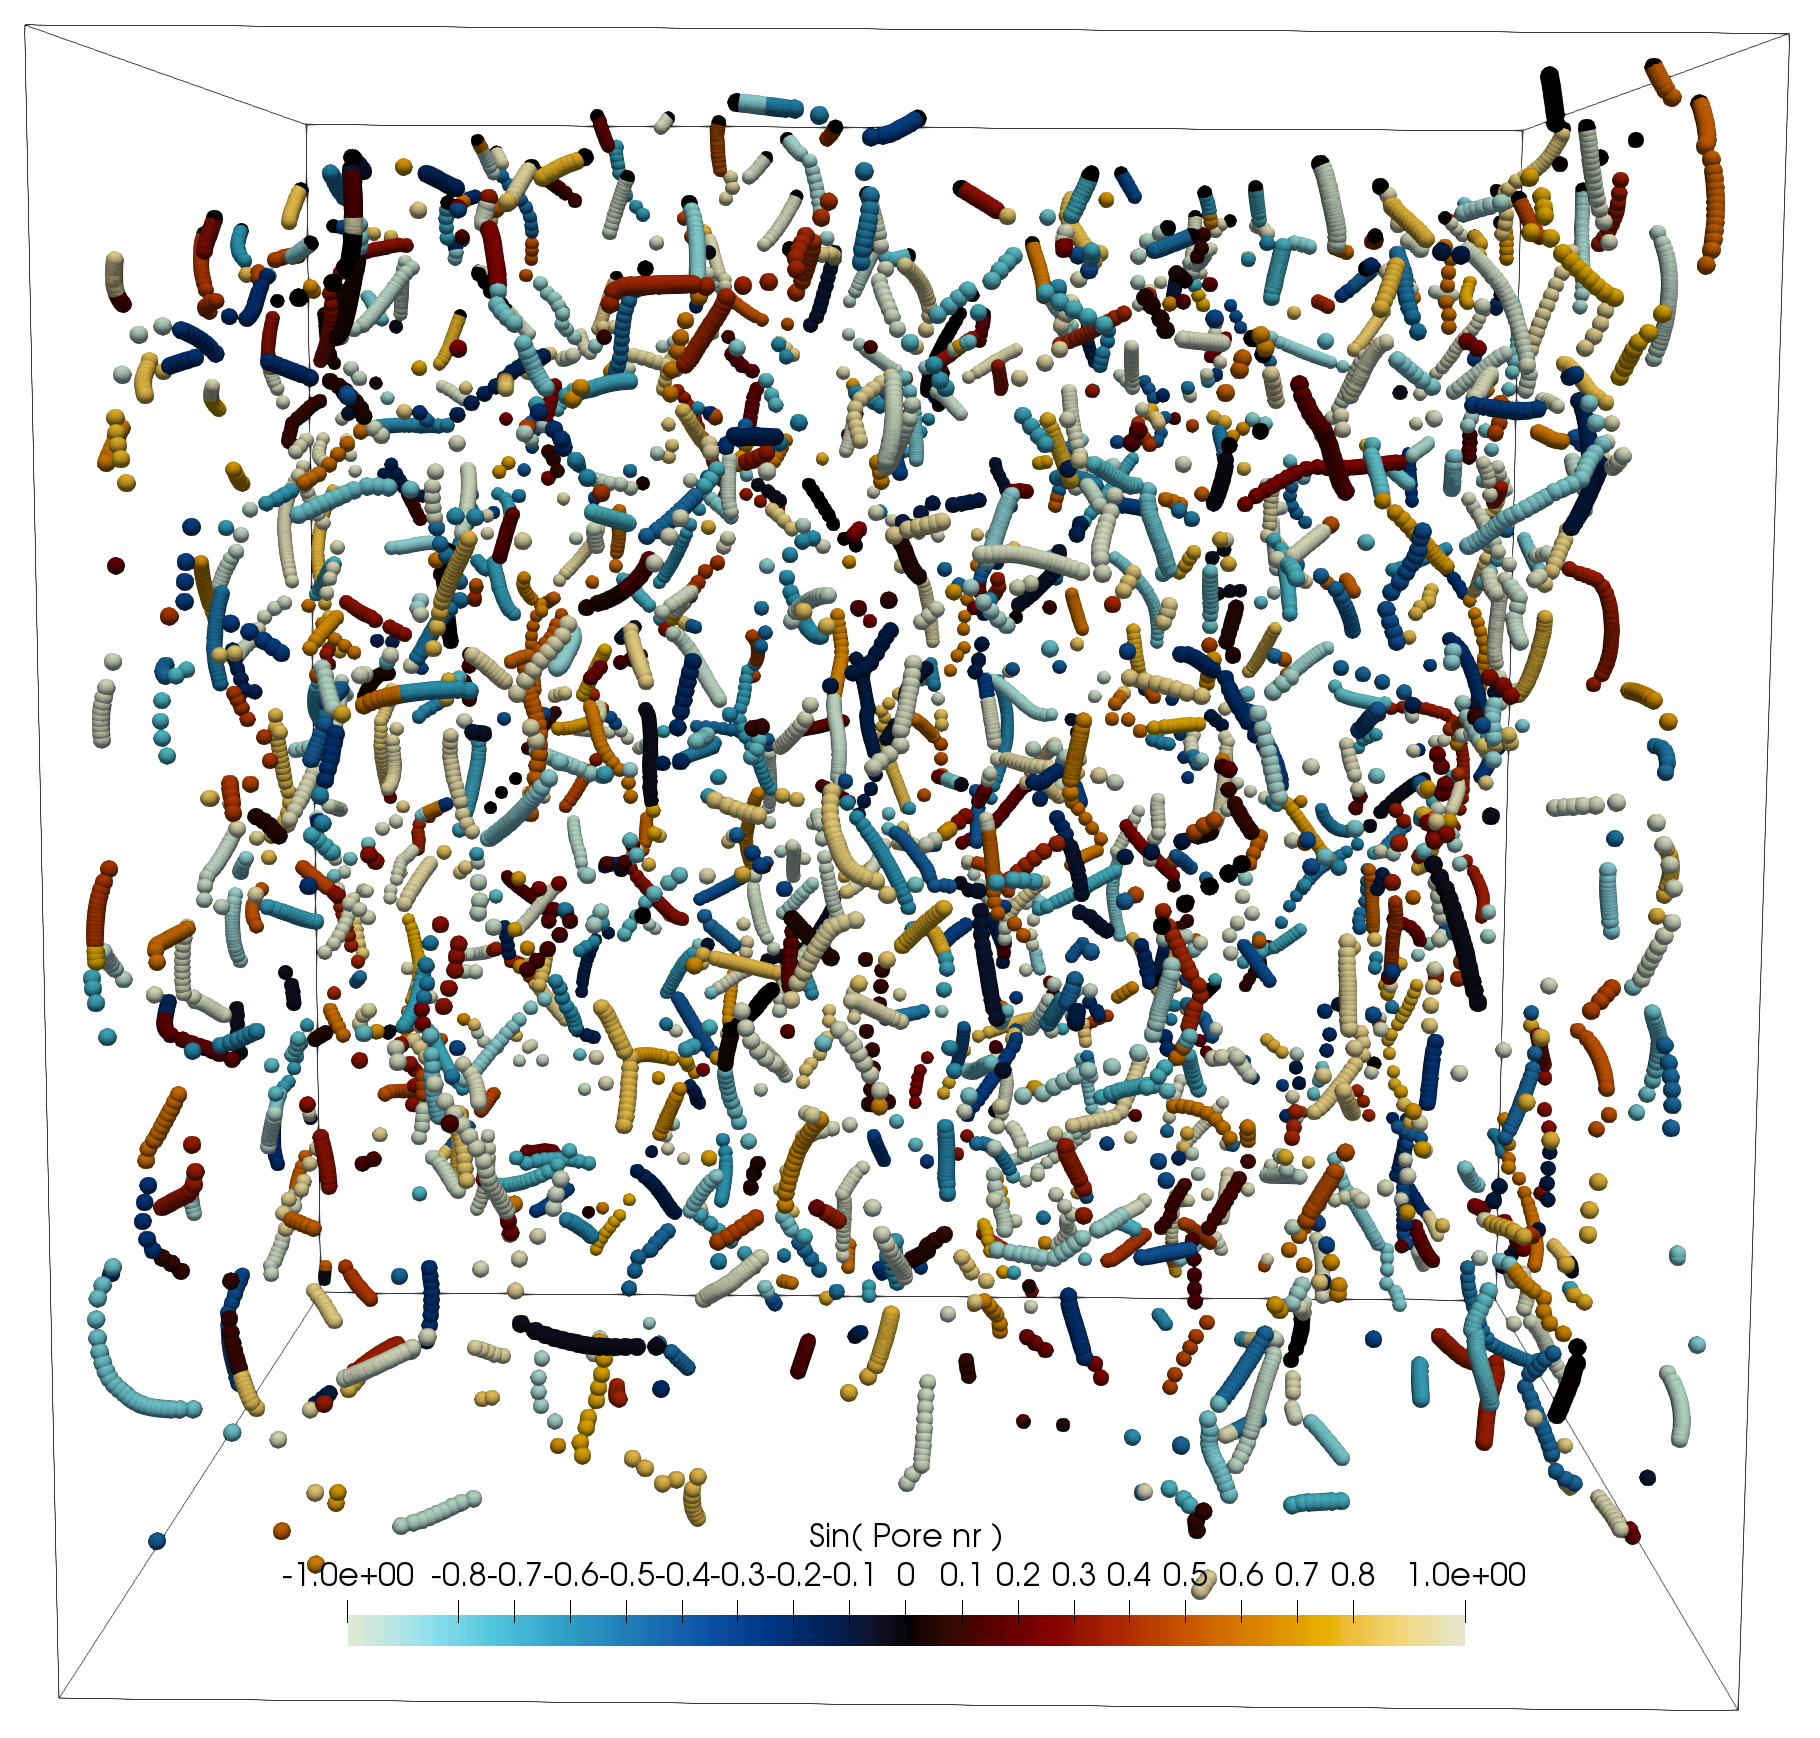
\includegraphics[height=5cm]{figures/pores_PM2.png}
\caption{Visualization of left: velocity field $|\mathbf{u}|$of an iso-pressure surface $\mathcal{S}(p)$ at pressure value $p$, middle: segmentation into iso-pressure patches  $\mathcal{S}_i(p)$, right: Pore identification throughout the porous medium. }\label{fig:segmentation}
\end{figure}


\subsection{Extraction of pores based on iso-pressure surfaces}
A chain of VTK-based image analysis techniques \citeA{schroeder_visualization_2006,hernderson_paraview_2007} is employed to extract iso-pressure surfaces. The analysis is scripted with pvpython which comes with the Topology ToolKit (TTK) installation for MACOS High Sierra (python 2.7.15, Paraview 5.4.1, TTK 0.9.3) \cite{tierny_topology_2018}. Specific Paraview/TTK filters are denoted with a capital letter. Values for parameters are given without units, but can be inferred from its definition. Note that the results of the simulation assign $p$ with the kinematic pressure, i.e. in units $\rm{m^2s^{-2}}$, from which the derive the static pressure by multiplication with the fluid density $p_s = p\rho_{f}$. The results in the paper are in correct units (using $\rm{Pa}$ for $p$), but in the following keep $p$ as the kinematic pressure. 

\noindent\textbf{Iso-pressure surfaces $\mathcal{S}(p)$ and noise removal}
\begin{itemize}
	\item[-]The iso-pressure surfaces $\mathcal{S}(p)$ are obtained by taking a contour (Contour) filter on pressure value $p$ on the DNS data. For porous media 1 and 2 we have chosen $k$ iso-pressure surfaces $p_k = p_0+ k \delta p$ with $ \delta p= 5\times 10^{-6}$. Due to large heterogeneity in the pressure gradient in the third porous media we have chosen to double its resolution to $\delta p = 2.5\times 10^{-6}$. Due to the noisy edges, as described in the paper, we remove small area patches. This is done by segmenting $\mathcal{S}(p_k)$ with the Connectivity filter in $j\in \{1,M_k\}$ disconnected patches $\mathcal{S}_j(p_k)$ with total area $A_0(p_k)$. Each patch is isolated by a Threshold filter and its surface area $A_j(p_k)$ determined by an IntegrateVariables filter. A maximum value for $A_j(p_k)> A_{\rm{min}}$ is used to append (AppendGeometry) to construct $\mathcal{S}(p_k)$ with total area $A_{total}$ consisting of $N_k$ iso-pressure surface patches. The value  $A_{\rm{min}}$ is determined by a sensitivity study on the total remaining area $A_k$ and the number $N_k$ of remaining patches as a function of $ A_{\rm{min}}$. The threshold values are $A_{\rm{min}} = 3\times10^{-11}, 5\times10^{-11} $ and $2\times10^{-12}$ for the PM respectively and are determined from Fig.~ S2 showing $A_{\rm{total}}/A_0$ and $N/A_0$ as a function of $A_{\rm{min}}$ for three independent values of $p_k$. An example of $\mathcal{S}_i$ is shown in Fig. \ref{fig:segmentation} (left). The reduction of the total area has been at most $1.5\%$ for these three test iso-pressure surfaces.
	\item[-]For $i=0$ and $i=N$, the iso-pressures surfaces are flat. Since we deem this to be a finite size effect and in this case `unnatural' we allow the iso-pressure surfaces to develop over the first and last $10$ slices, defining $p_0$.
	\item[-]To repair some of the irregularities in the surface mesh we employ three more filters: Tetrahydralize, CleantoGrid, and an ExtractSurface.
\end{itemize}
\noindent\textbf{Segmentation of $\mathcal{S}_i(p_k)$}
\begin{itemize} 
	\item[-]To segment $\mathcal{S}_i(p_k)$ into $i\in{1,N_k}$ individual pores $\mathcal{S}_i(p_k)$ a connectivity filter is applied (Connectivity, enumeration named `RegionId'), followed by a ExtractSurface and GenerateSurfaceNormals filter. An example of a segmentation is shown in Fig. S1 (middle).
	\item[-] To obtain the circularity $\mathcal{C}_i(p_k)$ we take a Contour on numerically zeros velocity $|u|= 10^{-9}~\rm{m/s}$. The obtained contour is subsequently integrated to obtain $\mathcal{L}_i(p_k)$. 

	By visual inspection of the isopressure surfaces (using Paraview software) we see that the circumferences are irregular and will lead to an overestimation of $\mathcal{C}_i(p_k)$. To investigate the dependency of $\mathcal{L}$ on the magnitude  $|u|$ we performed a sensitivity study, see Fig.(S2). We found that although the circumferences are visually smoother for higher values of $|u|$ (See third row of Fig S2), fundamental shape features get lost before the smoothing is significant, and can therefore not be used. Choosing $|u|= 10^{-9}~\rm{m/s}$ gives us the closest boundary representation of the porous media boundary wall. 

	To get an estimate for the error of overestimating  of $\mathcal{C}_i(p_k)$, we have done a control study by comparing the circumference obtained by thresholding the porous media boundary directly on pressure $p_k$. This yields a total circumference of isopressure surface $\mathcal{S}(p_k)$. Comparing this to $\sum_i^{N(k)}\mathcal{C}_i(p_k)$, with $N(k)$ the total number of iso-pressure pathces of iso-pressure surface $\mathcal{S}(p_k)$, gives us an averaged overestimation of $\mathcal{C}_i(p_k)$  by a factor $\epsilon = 1.15\pm.01 ,~1.11\pm.01,$ and $~1.08\pm.04$, for the three porous media respectively. This estimate is based on $40$ iso-pressure surfaces taken from each porous media. 

	\item[-] For each $\mathcal{S}_i(p_k)$ we integrate (IntegrateVariables) the surface to extract the averaged position $\mathrm{X}_i(p_k)$, total flux $Q_i(p_k) = \int_{\mathcal{S}_i(p_k)}\mathbf{u}\cdot\mathbf{n}\,da$, and total area $A_{i,j}= \int_{\mathcal{S}_i(p_k)}da$ and circularity $\mathcal{C}_i(p_k) = \mathcal{L}^2_i(p_k)/(4\pi A_i(p_k))$. 
\end{itemize}



\begin{figure}
\setfigurenum{S2} %%You can change number for each figure if you want, not required. "S" prepended automatically.
\noindent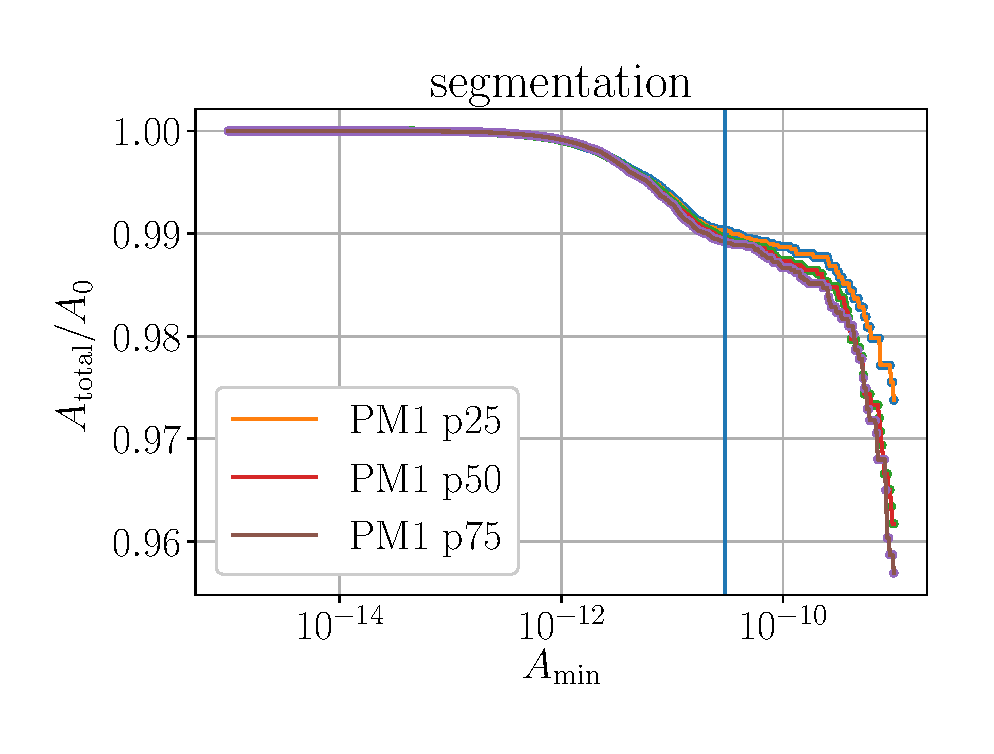
\includegraphics[height=4cm]{figures/SI_figures/segm_A_vs_Amin_PM1.eps}
\noindent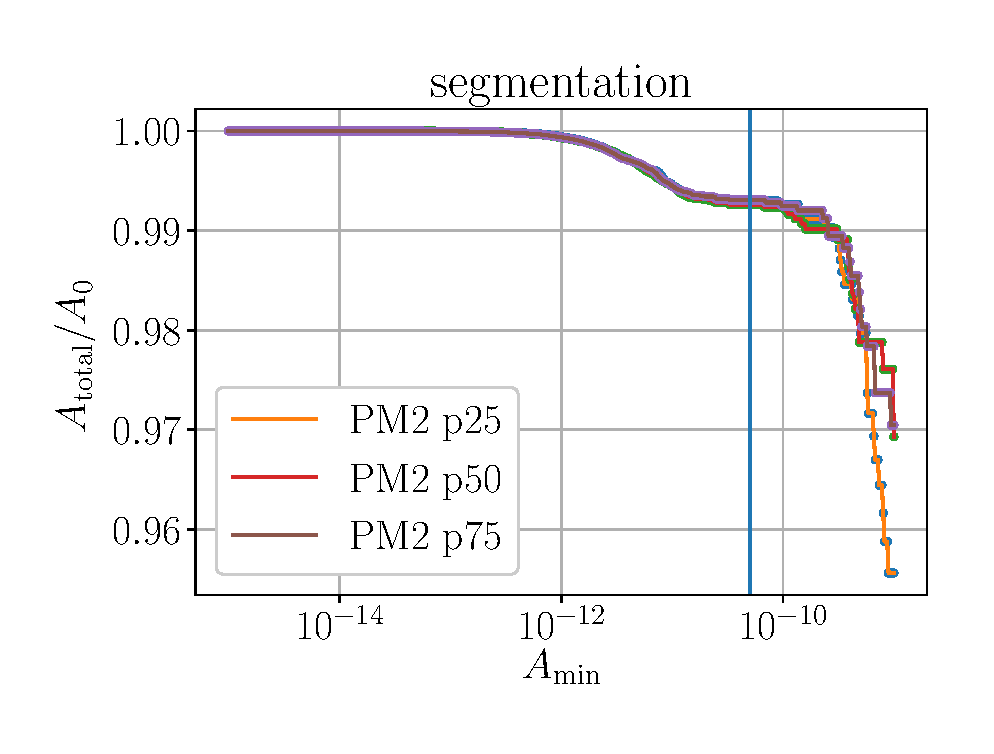
\includegraphics[height=4cm]{figures/SI_figures/segm_A_vs_Amin_PM2.eps}
\noindent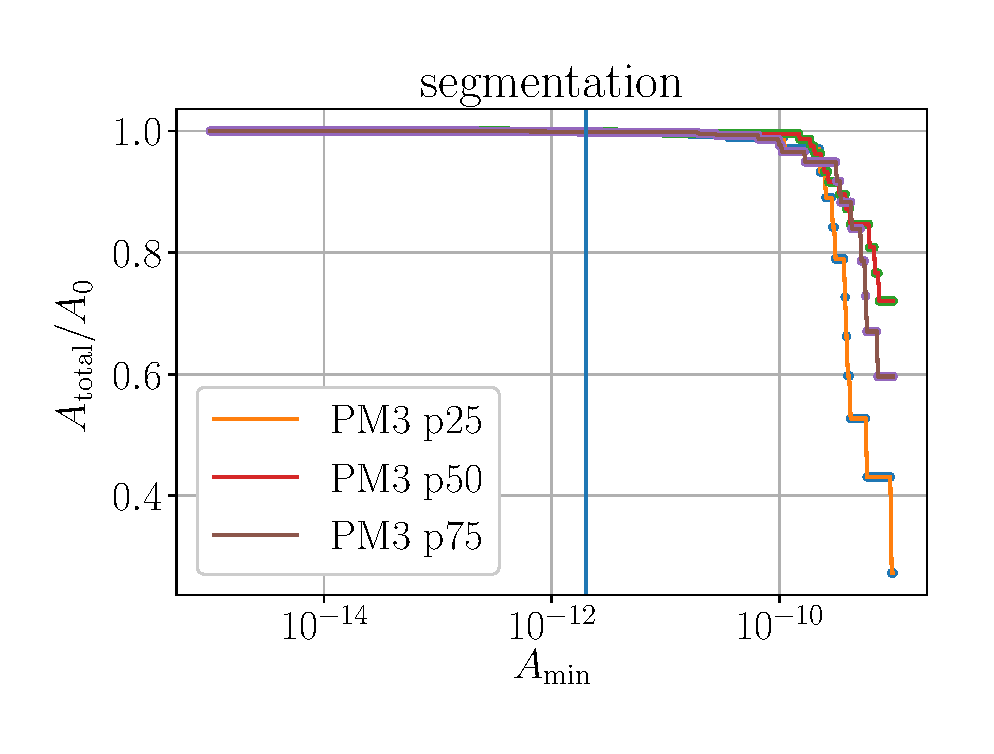
\includegraphics[height=4cm]{figures/SI_figures/segm_A_vs_Amin_PM3.eps}\\
\noindent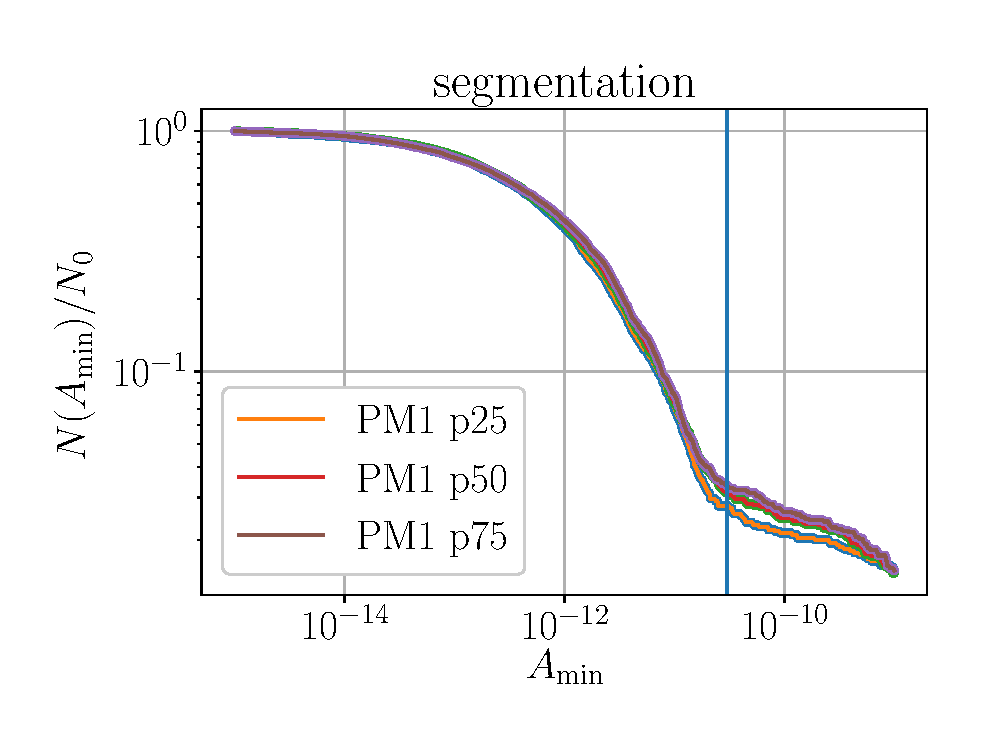
\includegraphics[height=4cm]{figures/SI_figures/segm_N_vs_Amin_PM1.eps}
\noindent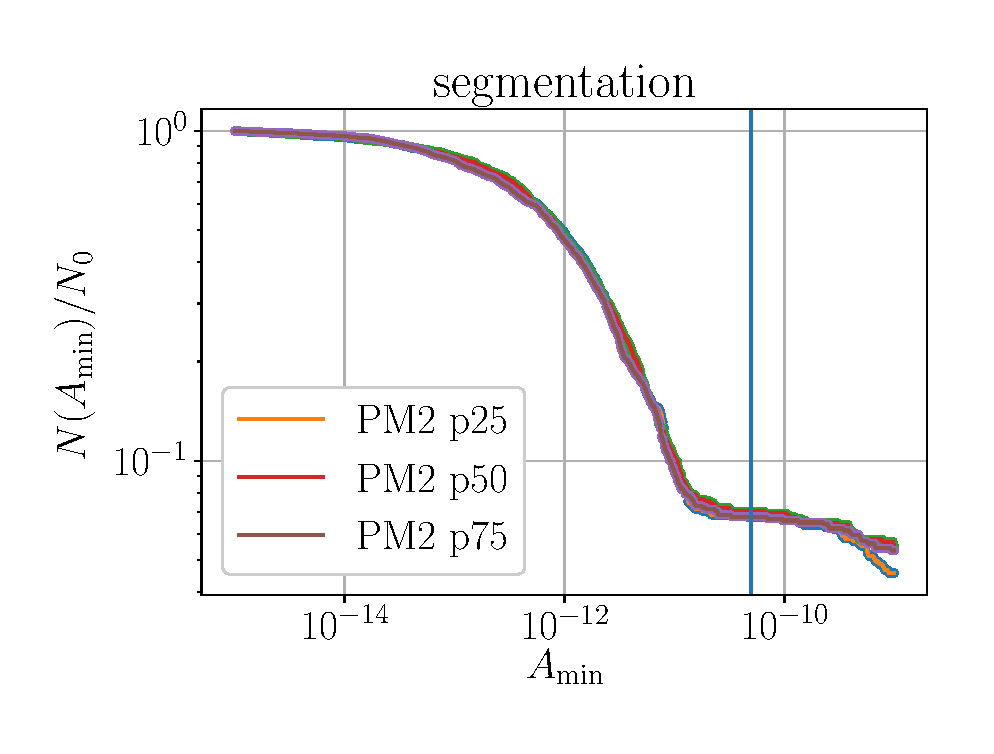
\includegraphics[height=4cm]{figures/SI_figures/segm_N_vs_Amin_PM2.eps}
\noindent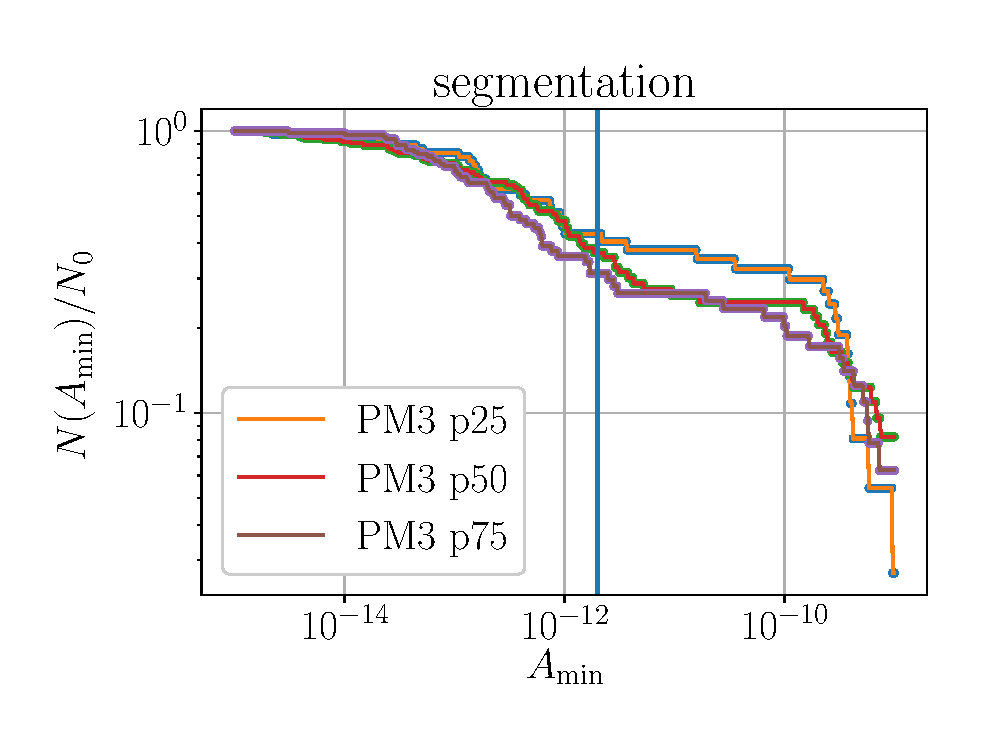
\includegraphics[height=4cm]{figures/SI_figures/segm_N_vs_Amin_PM3.eps}\\
\noindent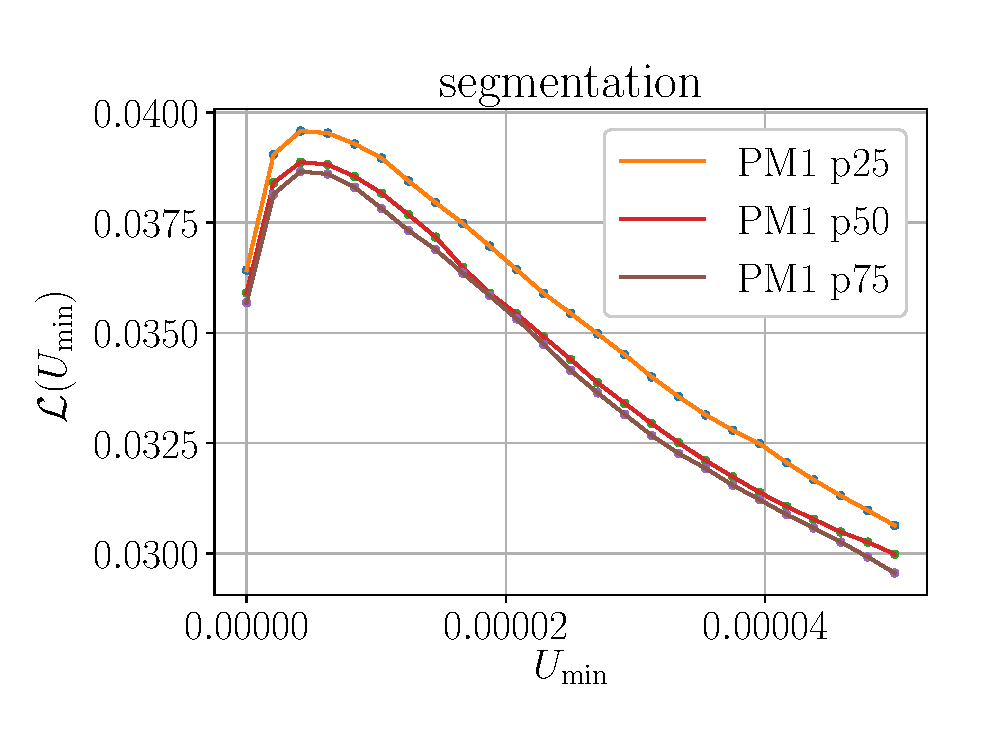
\includegraphics[height=4cm]{figures/SI_figures/L_vs_Umin_PM1.eps}
\noindent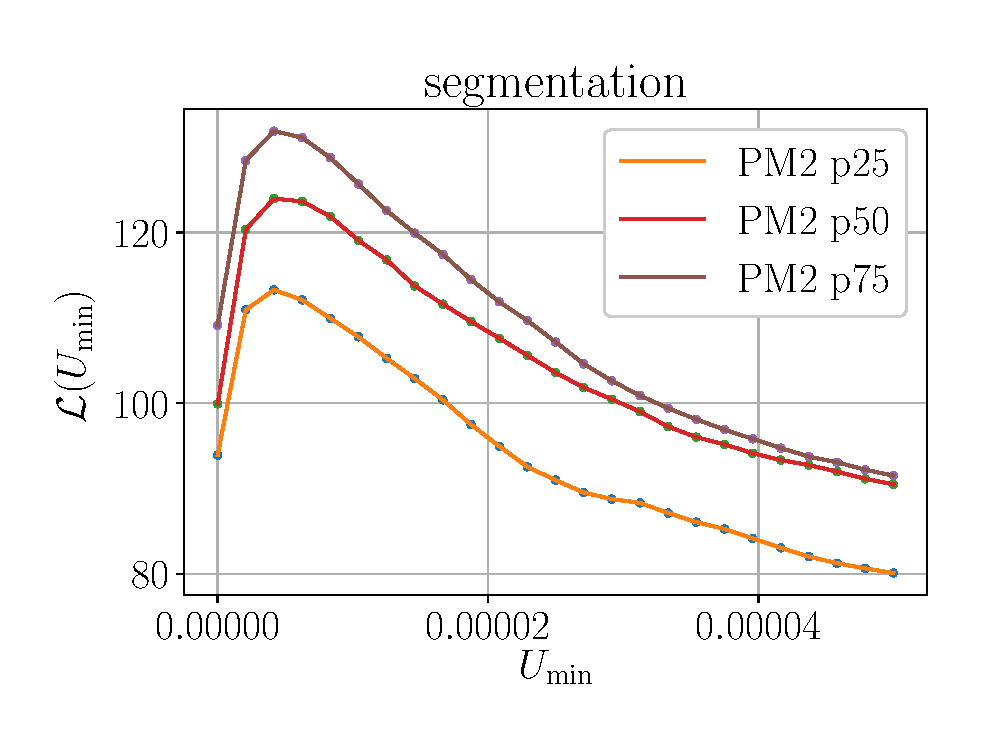
\includegraphics[height=4cm]{figures/SI_figures/L_vs_Umin_PM2.eps}
\noindent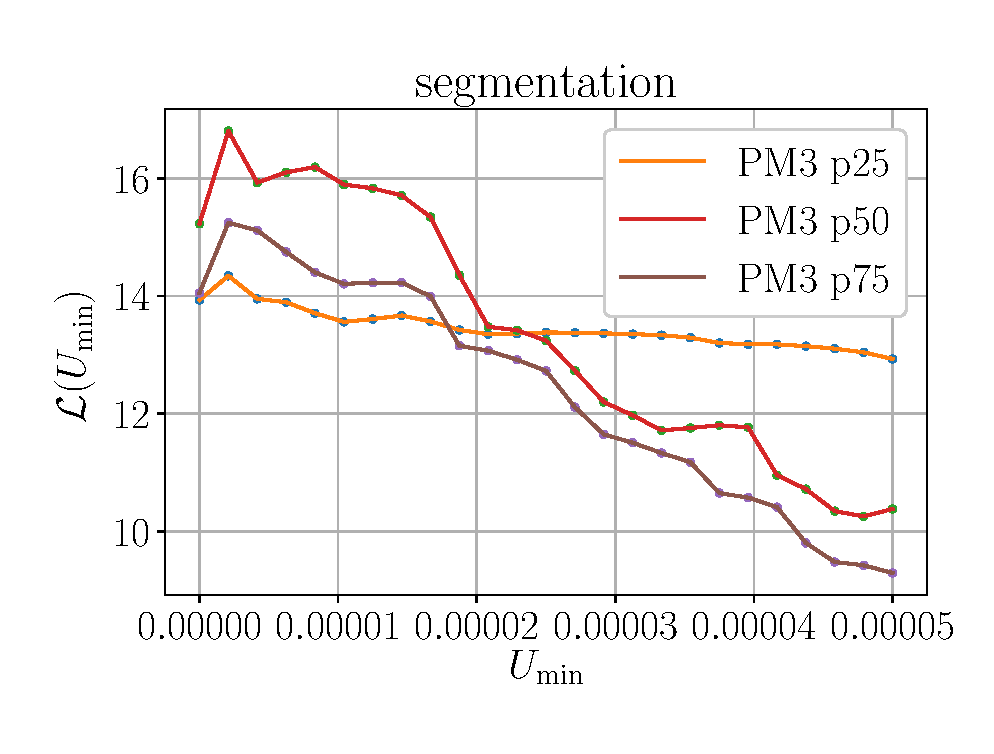
\includegraphics[height=4cm]{figures/SI_figures/L_vs_Umin_PM3.eps}\\
\noindent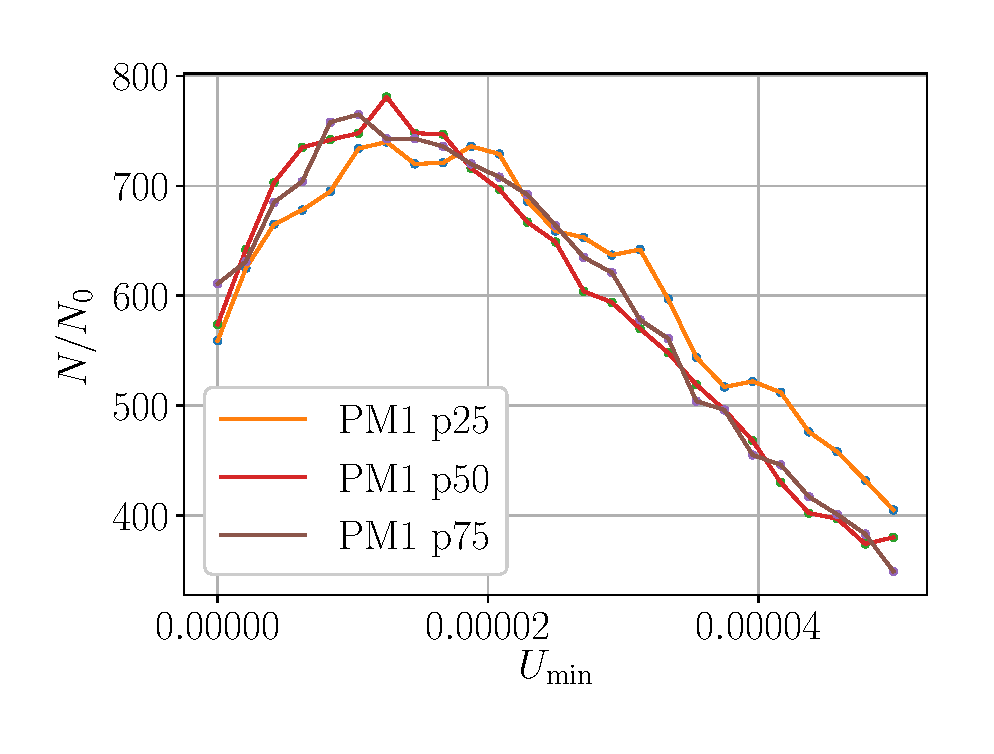
\includegraphics[height=4cm]{figures/SI_figures/N_vs_Umin_PM1.eps}
\noindent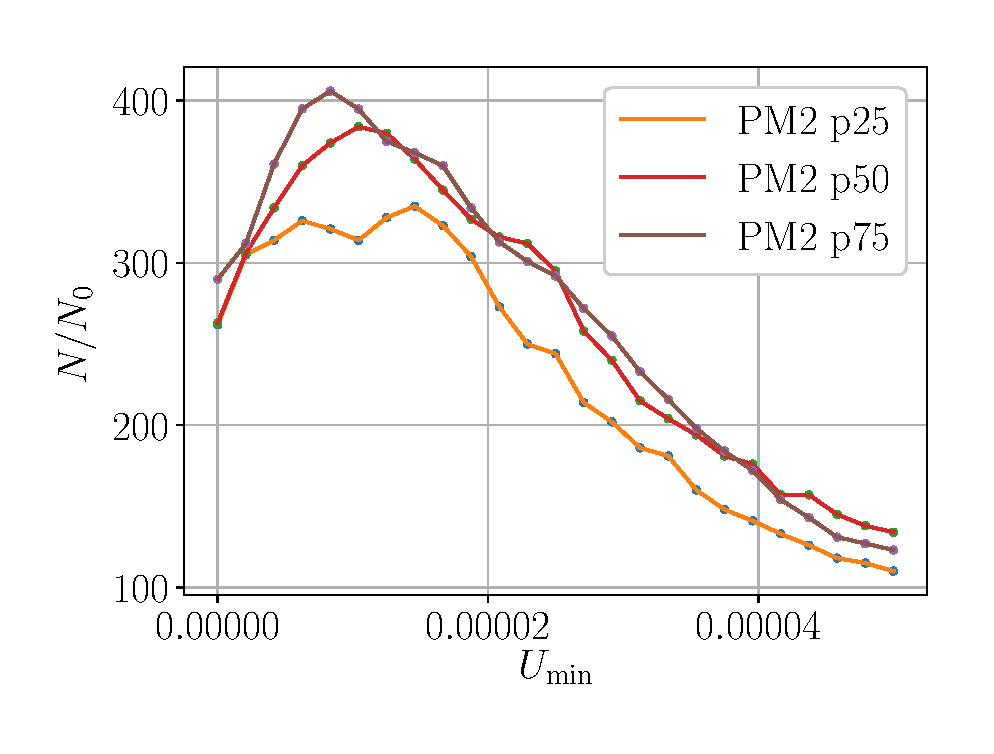
\includegraphics[height=4cm]{figures/SI_figures/N_vs_Umin_PM2.eps}
\noindent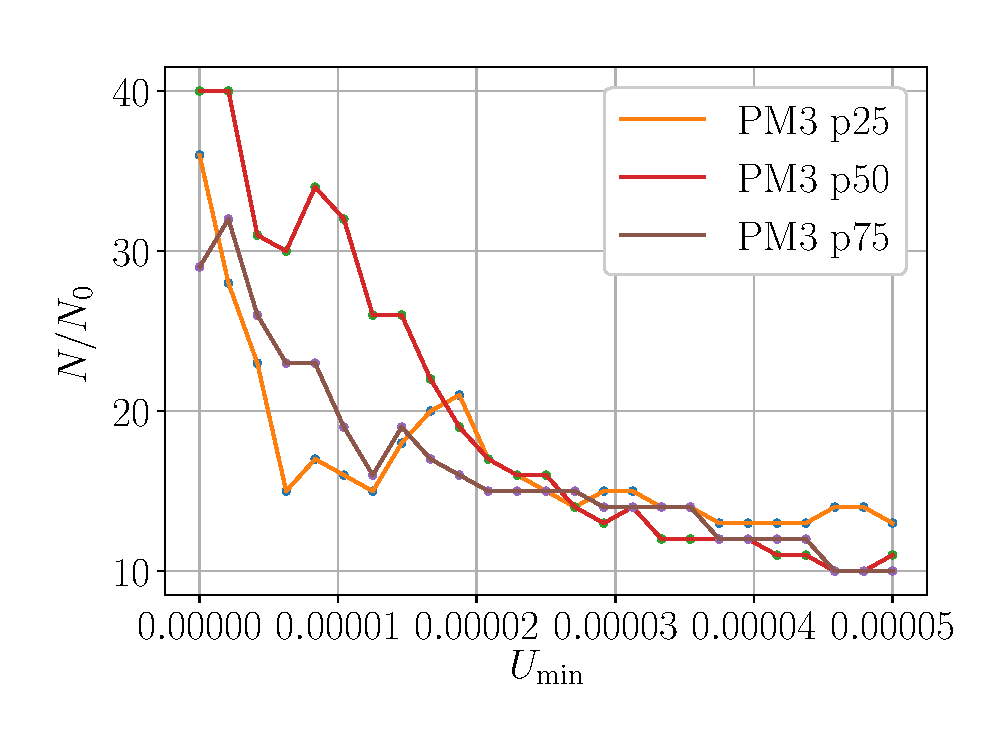
\includegraphics[height=4cm]{figures/SI_figures/N_vs_Umin_PM3.eps}
\caption{First row: Sensitivity study of total area $A$ as a function of $A_{\rm{min}}$. Second row:  Sensitivity study of the number of patches $N$ as a function of $A_{\rm{min}}$. Third row:  Sensitivity study of the total length of the circumference of three the iso-pressure surfaces $\mathcal{S}(p)$, $\mathcal{L}$ as a function of $\epsilon = U_{\rm{min}}$. Fourth row: Sensitivity study of the total number of iso-pressure `patches' $\mathcal{S}_i(p)$, $N$ as a function of $\epsilon = U_{\rm{min}}$.}
\end{figure}


% \begin{figure}
% \setfigurenum{S3} %%You can change number for each figure if you want, not required. "S" prepended automatically.
% \noindent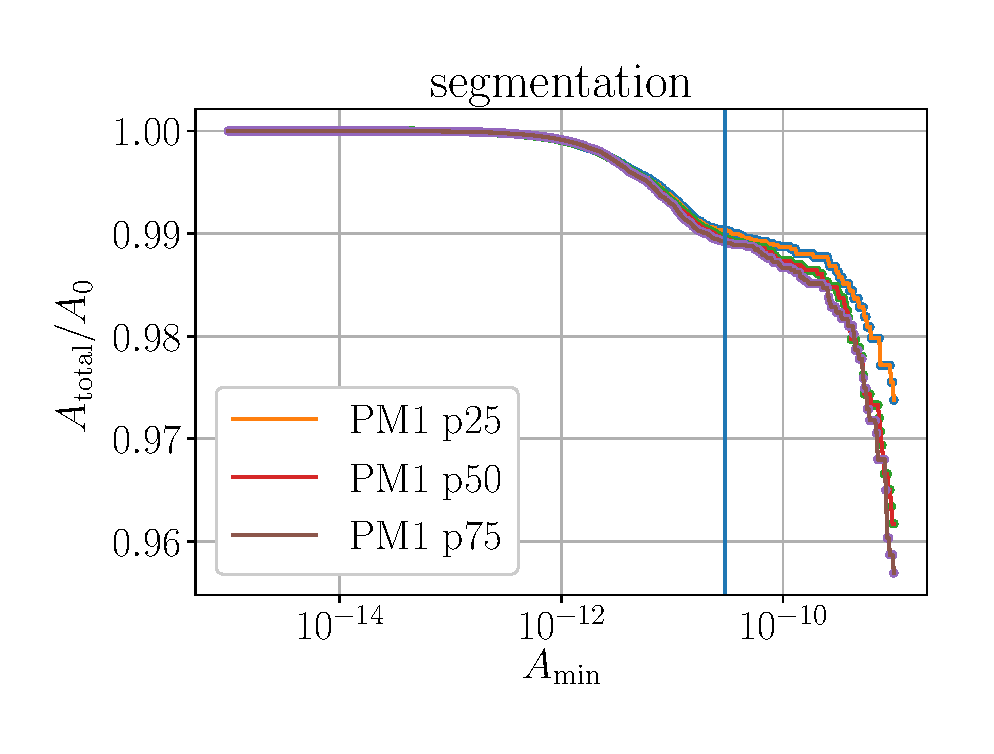
\includegraphics[height=4cm]{figures/SI_figures/segm_A_vs_Amin_PM1.eps}

% \caption{The irregularity of $\mathcal{L}$ as a function of three values of $\epsilon = U_{\rm{min}}$.}
% \end{figure}


\noindent\textbf{Local inheritance $\mathcal{S}_i(p)$}

Goal: For each $\mathcal{S}_i(p_k)$ finding its closest neighbor $\mathcal{S}_j(p_k+\delta p)$.  
\begin{itemize}
	\item[-]]This neighboring iso-pressure patch (building up a pore) is found by calculating the distance function $f_d(\mathbf{x},\mathcal{S})$, between point $\mathbf{x}\in \mathcal{S}_i(p_k)$ and all iso-pressure patches $\mathcal{S}_l(p_k+dp)$. This distance function is calculated by the vtkDistancePolyDataFilter, a programmable vtk filter, and is defined by 
		\begin{equation}
			f_d\left(\mathbf{x},\mathcal{S}\right) = \min \{\Vert\mathbf{x}-\mathbf{y}\Vert \} ~|~ \mathbf{y}\in \mathcal{S}.
		\end{equation}
	for each $i,l$ we define the averaged distance matrix by using the IntegrateVariables filter
		\begin{equation}
			d_{i,l}(p_k) = \frac{1}{A_i(p_k)}\int_{\mathcal{S}_i(p_k)} f_d(\mathbf{x}_i,\mathcal{S}_l(p_k+\delta p)) \,dS_i.
		\end{equation}
	The closest neighbor $\mathcal{S}_j(p_k+\delta p)$ is found by the minimum value of $d_{i,j}(p_k) = \rm{min}\left\{ d_{i,l}(p_k)\right\}$. The closest neighbor is assigned by the identification number of the nearest neighbor $n_i(p_k) = j$ 
	\item[-] Subsequently we compute the change in surface area $dA_i(p_k) = A_i(p_k)-A_j(p_k+\delta p)$, the averaged location of the neighboring pore $\mathbf{X}^n_i(p_k) = \mathbf{X}_j(p_k+\delta p)$ and the distances between the two averaged coordinates $dX_i(p_k) = \left| \mathbf{X}_i(p_k)-\mathbf{X}_j(p_k+\delta p)\right|$. Last but not least we assign $dx_i(p_k) = d_{i,j}(p_k)$, which is used as $dx$ in the Eq. (10) and (12).
	\item[-] Now each patch $\mathcal{S}_i(p_k)$ has intrinsic attributes enlisted: $i, n_i, \mathbf{X}_i$, $Q_i$, $A_i$, $\mathcal{C}_i$. Additionally it has attributes that depend on its nearest neighbor $n_i$, $\mathbf{X}^n_i$, $dA_i$, $dx_i$ and $dX_i$. For all these attributes $p_k$ is implied. The intrinsic attributes of the nearest neighbor are added to the attributes of $\mathcal{S}_i(p_k)$ for convenience. 
	\item[-] It is important to notice the difference between $dx_i$ and $dX_i$. The former is the averaged distance between two iso-pressure surface patches and therefore assigned to $dx$ wich stems from $dV = Adx$. The latter is the distance between the two averaged positions of the iso-pressure patches. 
	\item[-]Gathered all necessary pore attributes, we can use a least-squared fit of Eq.(9) to obtain $\alpha_i$ and Eq.(15) to obtain $\alpha$ and $\beta$. 
\end{itemize}


\noindent\textbf{Defining pores by integration of local inheritance of $\mathcal{S}_i(p)$}
\begin{itemize}
	\item For the first iso-pressure patches $S_i(p_0)$ we initiate a pore identification number $P_i(p_k) = i$. 
	\item For each pore $i$ we integrate to the nearest neighbor $j$ by assigning the same pore number to $\mathcal{S}_{n_i}(p_0+\delta p)$ : $P_{n_i}(p_0+\delta p) = i$. This forward integration takes place only when five quality factors are fulfilled,
	\item $Q_1 = (|dX_i-dX_{n_i}|)/dX_i<q_1$: Ensuring that there is no abrupt change in consecutive averaged distances. 
	\item $Q_2 = |dA_i|/A_i<q_2$: Ensuring no abrupt changes in the surface area of consecutive area patches. 
	\item $Q_3 = (|Q_{0,j}-Q_{1,nn_{i,j}}|)/Q_{1,nn_{i,j}}<q_3$: Ensuring that the flux is `nearly' conserved.  
	\item $Q_4 = dX_i < q_4$: Ensuring that pores split if they are too far apart. 
	\item $Q_5 = A_i > q_5$: Removing `small' area patches. 
	The values are found by trial and error to decrease the number of pores but still capturing the merging and splitting of pores. For each quality factor we have 3 values tailored to each porous media 1,2 and 3 independently. For $q_1 = [1.6,.4,.4]$
, $q_2 = [.5,.5,1]$, $q_3 = [.2,.2,1]$, $q_4 = [10^{-5},10^{-5},9\times10^{-5}]$ and $q_5 = [1\times10^{-10},1\times10^{-10},5\times10^{-11}]$	These requirement seem quite loose, but have proven to be quite effective. 
	\item The assignment of pore numbers can continue iteratively until all patches have a pore identification number $P_i(p_k)$.	
	\item[-]For all $P_i$ we can calculate Eq.(12) and Eq.(15).
\end{itemize}



\section{Fitting models, Results and Performance}
\subsection{Fitting models}
In the paper we have fitted four models $f_i$ 
\begin{equation}
	\frac{dp}{dx} = \frac{Q}{A^2} f_i
\end{equation}
for all consecutive pore patches that comply with the the quality factors $Q_i$, not to be mistaken with averaged flux. Since the data is spread over multiple orders of magnitude, we obtained a least squared fit by taking the logarithm on either side of the equation
\begin{equation}
	\log{\left[\frac{dp}{dx}\right]} = \log{\left[\frac{Q}{A^2} f_i\right]}
\end{equation}
The 4 functions that have been fitted are given by 
\begin{eqnarray*}
	f_{\rm{HP}} =&  1~~~~~~~~~~~~~~~~~~~~~~~~~~~~ \\
	f_1 =&  \alpha_0+\alpha_1\mathcal{C} + \alpha_2 \frac{1}{A}\left|\frac{d A}{d x}\right|^2\\
	f_2 =&  \beta_0+\beta_1\mathcal{C} ~~~~~~~~~~~~~~~~~~~\\
	f_3 =& 1-\alpha\left[1-\left(\mathcal{C}/\epsilon\right)^{\beta}\right].~~~~~~~~~~\\
	f_4 =& \gamma_0+\gamma_1\left(\mathcal{C}/\epsilon\right)+\gamma_1\left(\mathcal{C}/\epsilon\right)^2.~~~~~~~~~~
\end{eqnarray*}

For $f_3$ and $f_4$ we have used an overall correction factor for $\mathcal{C}$ specific to each porous media as reported in the paper. We have included one additional condition that $dp/dx > 0.8 \frac{Q}{A^2}$, to ensure that unphysical measurements of the pressure gradient. This can be caused by wrongly matched patches. This led to a reduction in evaluated surface areas of $0.4\%$, $0.3\%$ and $2.6\%$ for the porous media respectively. In addition singular patches that have not been matches are contributing to respectively $18\%, 26\%$ and $1.7\%$ of the evaluated surface areas. 

\subsection{Results 1}

Summary of fitting parameters and error measures for porous media 1\\
\begin{tabular}{l|c|c|c}
\hline
model & parameters  & relative contributions & $R^2$  \\
\hline
$f_{\rm{HP}}$&-  									& $[100\%]$ &  $0.91$  \\
$f_1$		&$\alpha_0 = 0.48,~\alpha_1 = 0.90,~\alpha_2 = -6.3\times 10^{-7} $ 	& $[23\%,77\%,<.1\%]$ & $0.98$ \\
$f_2$ 		&$\beta_0 = 0.48,~\beta_1 = 0.90 $				&  $[23\%,77\%]$ & $0.97$\\
$f_3$ 		&$\alpha = 0.45,~\beta = 1.09 $					& -  & $0.97$\\
$f_4$ 		&$\gamma_0 = 0.53,~\gamma_1 = 1.18,~\gamma_2 = 9.5\times10^{-3} $ & $[25\%,73\%,1\%]$ & $0.98$\\
\end{tabular}

\vspace{1cm}

Summary of fitting parameters and error measures for porous media 2\\
\begin{tabular}{l|c|c|c}
\hline
model & parameters  & relative contributions & $R^2$  \\
\hline
$f_{\rm{HP}}$&-  									& $[100\%]$ &  $0.97$  \\
$f_1$		&$\alpha_0 = 0.52,~\alpha_1 = 0.87,~\alpha_2 = 1.1\times 10^{-6} $ 	& $[31\%,69\%,<.1\%]$ & $0.99$ \\
$f_2$ 		&$\beta_0 = 0.52,~\beta_1 = 0.87 $				&  $[31\%,69\%]$ & $0.99$\\
$f_3$ 		&$\alpha = 0.58,~\beta = 1.05 $					& -  & $0.98$\\
$f_4$ 		&$\gamma_0 = 0.71,~\gamma_1 = 0.65,~\gamma_2 = 0.06 $ & $[42\%,51\%,8\%]$ & $0.99$\\
\end{tabular}

\vspace{1cm}


Summary of fitting parameters and error measures for porous media 3\\
\begin{tabular}{l|c|c|c}
\hline
model & parameters  & relative contributions & $R^2$  \\
\hline
$f_{\rm{HP}}$&-  									& $[100\%]$ &  $0.94$  \\
$f_1$		&$\alpha_0 = 0.26,~\alpha_1 = 1.07,~\alpha_2 = 6.3\times 10^{-5} $ 	& $[18\%,82\%,<.1\%]$ & $0.97$ \\
$f_2$ 		&$\beta_0 = 0.26,~\beta_1 = 1.07 $				&  $[18\%,82\%]$ & $0.97$\\
$f_3$ 		&$\alpha = 0.34, \beta = 1.08 $					& -  & $0.97$\\
$f_4$ 		&$\gamma_0 = 2.1,~\gamma_1 = -2.1,~\gamma_2 = 1.4 $ & $[148\%,-136\%,88\%]$ & $0.96$\\
\end{tabular}

 
\subsection{Results 2}

The model performance have been expressed in the Pearson correlation coefficient $R^2$ of the measured $\mathcal{R}_{\rm{meas}}= \Delta p/Q$ and the modeled,

\begin{equation}
	\mathcal{R}_{\rm{m}}(f_i) = \int^{L_{\rm{eff}}}_{0}\frac{1}{A^2}f_i(\mathcal{C})\,dx,
\end{equation}

and the HP model 

\begin{equation}
	\mathcal{R}_{\rm{HP}} = \int^{L_{\rm{eff}}}_{0}\frac{1}{A^2}\,dx.
\end{equation}

Since the errors between $\mathcal{R}_{\rm{meas}}$ and $\mathcal{R}_{\rm{HP}}$ shows a high degree of heteroscedasticy \cite{wilcox_comparing_2009}, the Pearson correlation function is not adequate to compare these models, therefore we also computed the root-mean-square-relative error (RMSRE). To investigate the potential improvement on preferential channels (those with low resistances or high fluxes), we weighted the RMSRE with the total flux $Q$ through the pore, $\rm{RMSRE}_Q$. The results are shown in the following tables for the three porous media respectively. 

\noindent{\bf{Summary model hydraulic resistance performance for porous media 1:}}\\
\begin{tabular}{l|c|c|c}
\hline
model & $R^2$  & $\rm{RMSRE}$ & $\rm{RMSRE}_Q$  \\
\hline
$\mathcal{R}_{\rm{HP}}$ 	& $0.91$ & $0.59$ & $0.86$\\
$\mathcal{R}_{\rm{m}}(f_2)$	& $0.97$ & $0.12$ & $0.10$\\
$\mathcal{R}_{\rm{m}}(f_3)$	& $0.97$ & $0.32$ & $0.27$\\
\end{tabular}

\vspace{1cm}

\noindent{\bf{Summary model hydraulic resistance performance for porous media 2:}}\\
\begin{tabular}{l|c|c|c}
\hline
model & $R^2$  & $\rm{RMSRE}$ & $\rm{RMSRE}_Q$  \\
\hline
$\mathcal{R}_{\rm{HP}}$ 	& $0.88$ & $0.48$ & $0.61$\\
$\mathcal{R}_{\rm{m}}(f_2)$	& $0.95$ & $0.14$ & $0.13$\\
$\mathcal{R}_{\rm{m}}(f_3)$	& $0.95$ & $0.28$ & $0.29$\\
\end{tabular}

\vspace{1cm}
\noindent{\bf{Summary model hydraulic resistance performance for porous media 3:}}\\
\begin{tabular}{l|c|c|c}
\hline
model & $R^2$  & $\rm{RMSRE}$ & $\rm{RMSRE}_Q$  \\
\hline
$\mathcal{R}_{\rm{HP}}$ 	& $0.99$ & $0.32$ & $0.32$\\
$\mathcal{R}_{\rm{m}}(f_2)$	& $0.99$ & $0.17$ & $0.15$\\
$\mathcal{R}_{\rm{m}}(f_3)$	& $0.99$ & $0.28$ & $0.20$\\
\end{tabular}




\section{Measuring the relative Longitudinal and Transversal energy dissipation on an iso-pressure surface} 
In the theoretical section of the paper we have derived expressions for the longitudinal and transversal energy dissipation tensors, by 
\begin{equation}\label{eq:reduced_dissipation_tensor}
\left|\nabla_i u_j\right|^2 \approx  \left|\nabla_s u_p\right|^2 + \left|\nabla_n u_p\right|^2 .
\end{equation}
where we have assumed that the terms $ \left|\nabla_n u_n\right|^2$ and $ \left|\nabla_s u_n\right|^2$ are negligible. We will show two examples where we have calculated the individual terms of the total viscous dissipation. Because the highest dissipation is expected to be located near the porous media interface and the discretization also refined at the interface the numerical noise is also expected to be higher, see Fig\ref{fig:numerical noise}. All 3 porous media contain some points in the mesh where the VTK gradient filter can't factorize the linear system which leads to very high values of the respected fields. The origin lies likely in the mesh quality generated by the snappyHexMesh generator contained in the openFoam simulation. Since the simulations have all converged we do not question the original simulation results but we do note that post-processing of these meshes can be difficult especially if gradients have to be calculated. Nevertheless we have tried to quantify the relevance of the transversal and longitudinal terms of the viscous dissipation tensor. We have chosen to threshold the unreasonable high gradient terms based on outliers in the histograms of the gradients. For the first porous media the porous media the refinement was chosen a degree higher than the others, and led to `nan' results of the integrated relative contributions. For the two other porous media we have found reasonable results given in Table \ref{tab:sm1}. Since we have to filter out quit some data that exhibits unreasonable high values the percentages are not adding up to $100\%$. By visual inspection we can examine the term $\left|\nabla_i u_j\right|^2$ in all porous media and we see that the total dissipation correlates with gradients in the transverse direction. Also in this data we can see that for Porous Media 3 the relative contribution of the longitudinal term $ \left|\nabla_n u_p\right|^2$, $24\%$ is in the same order as the transversal term $ \left|\nabla_s u_p\right|^2$ which amounts to $32\%$. This observation is in agreement with the fitting of the two contributions in the paper.


\end{article}

\begin{table}[htbp!]\label{tab:sm1}
\centering
\begin{tabular}{l|c|c|c|c|c}
PM & & $\left|\nabla_s u_p\right|^2$ & $ \left|\nabla_n u_p\right|^2$ & $\left|\nabla_n u_n\right|^2$ & $\left|\nabla_n u_n\right|^2$ \\
\hline
PM2 &  & $71 \%$ & $17\%$ & $12\%$ & $12\%$ \\
PM3 &  & $32 \%$ & $24\%$ & $10\%$ & $5\%$ \\
\end{tabular}
\caption{\label{tab:table-name}Estimated relative contributions to the total viscous dissipation on an iso-pressure surface. }
\end{table}




\begin{figure}
\setfigurenum{S3} %%You can change number for each figure if you want, not required. "S" prepended automatically.
\noindent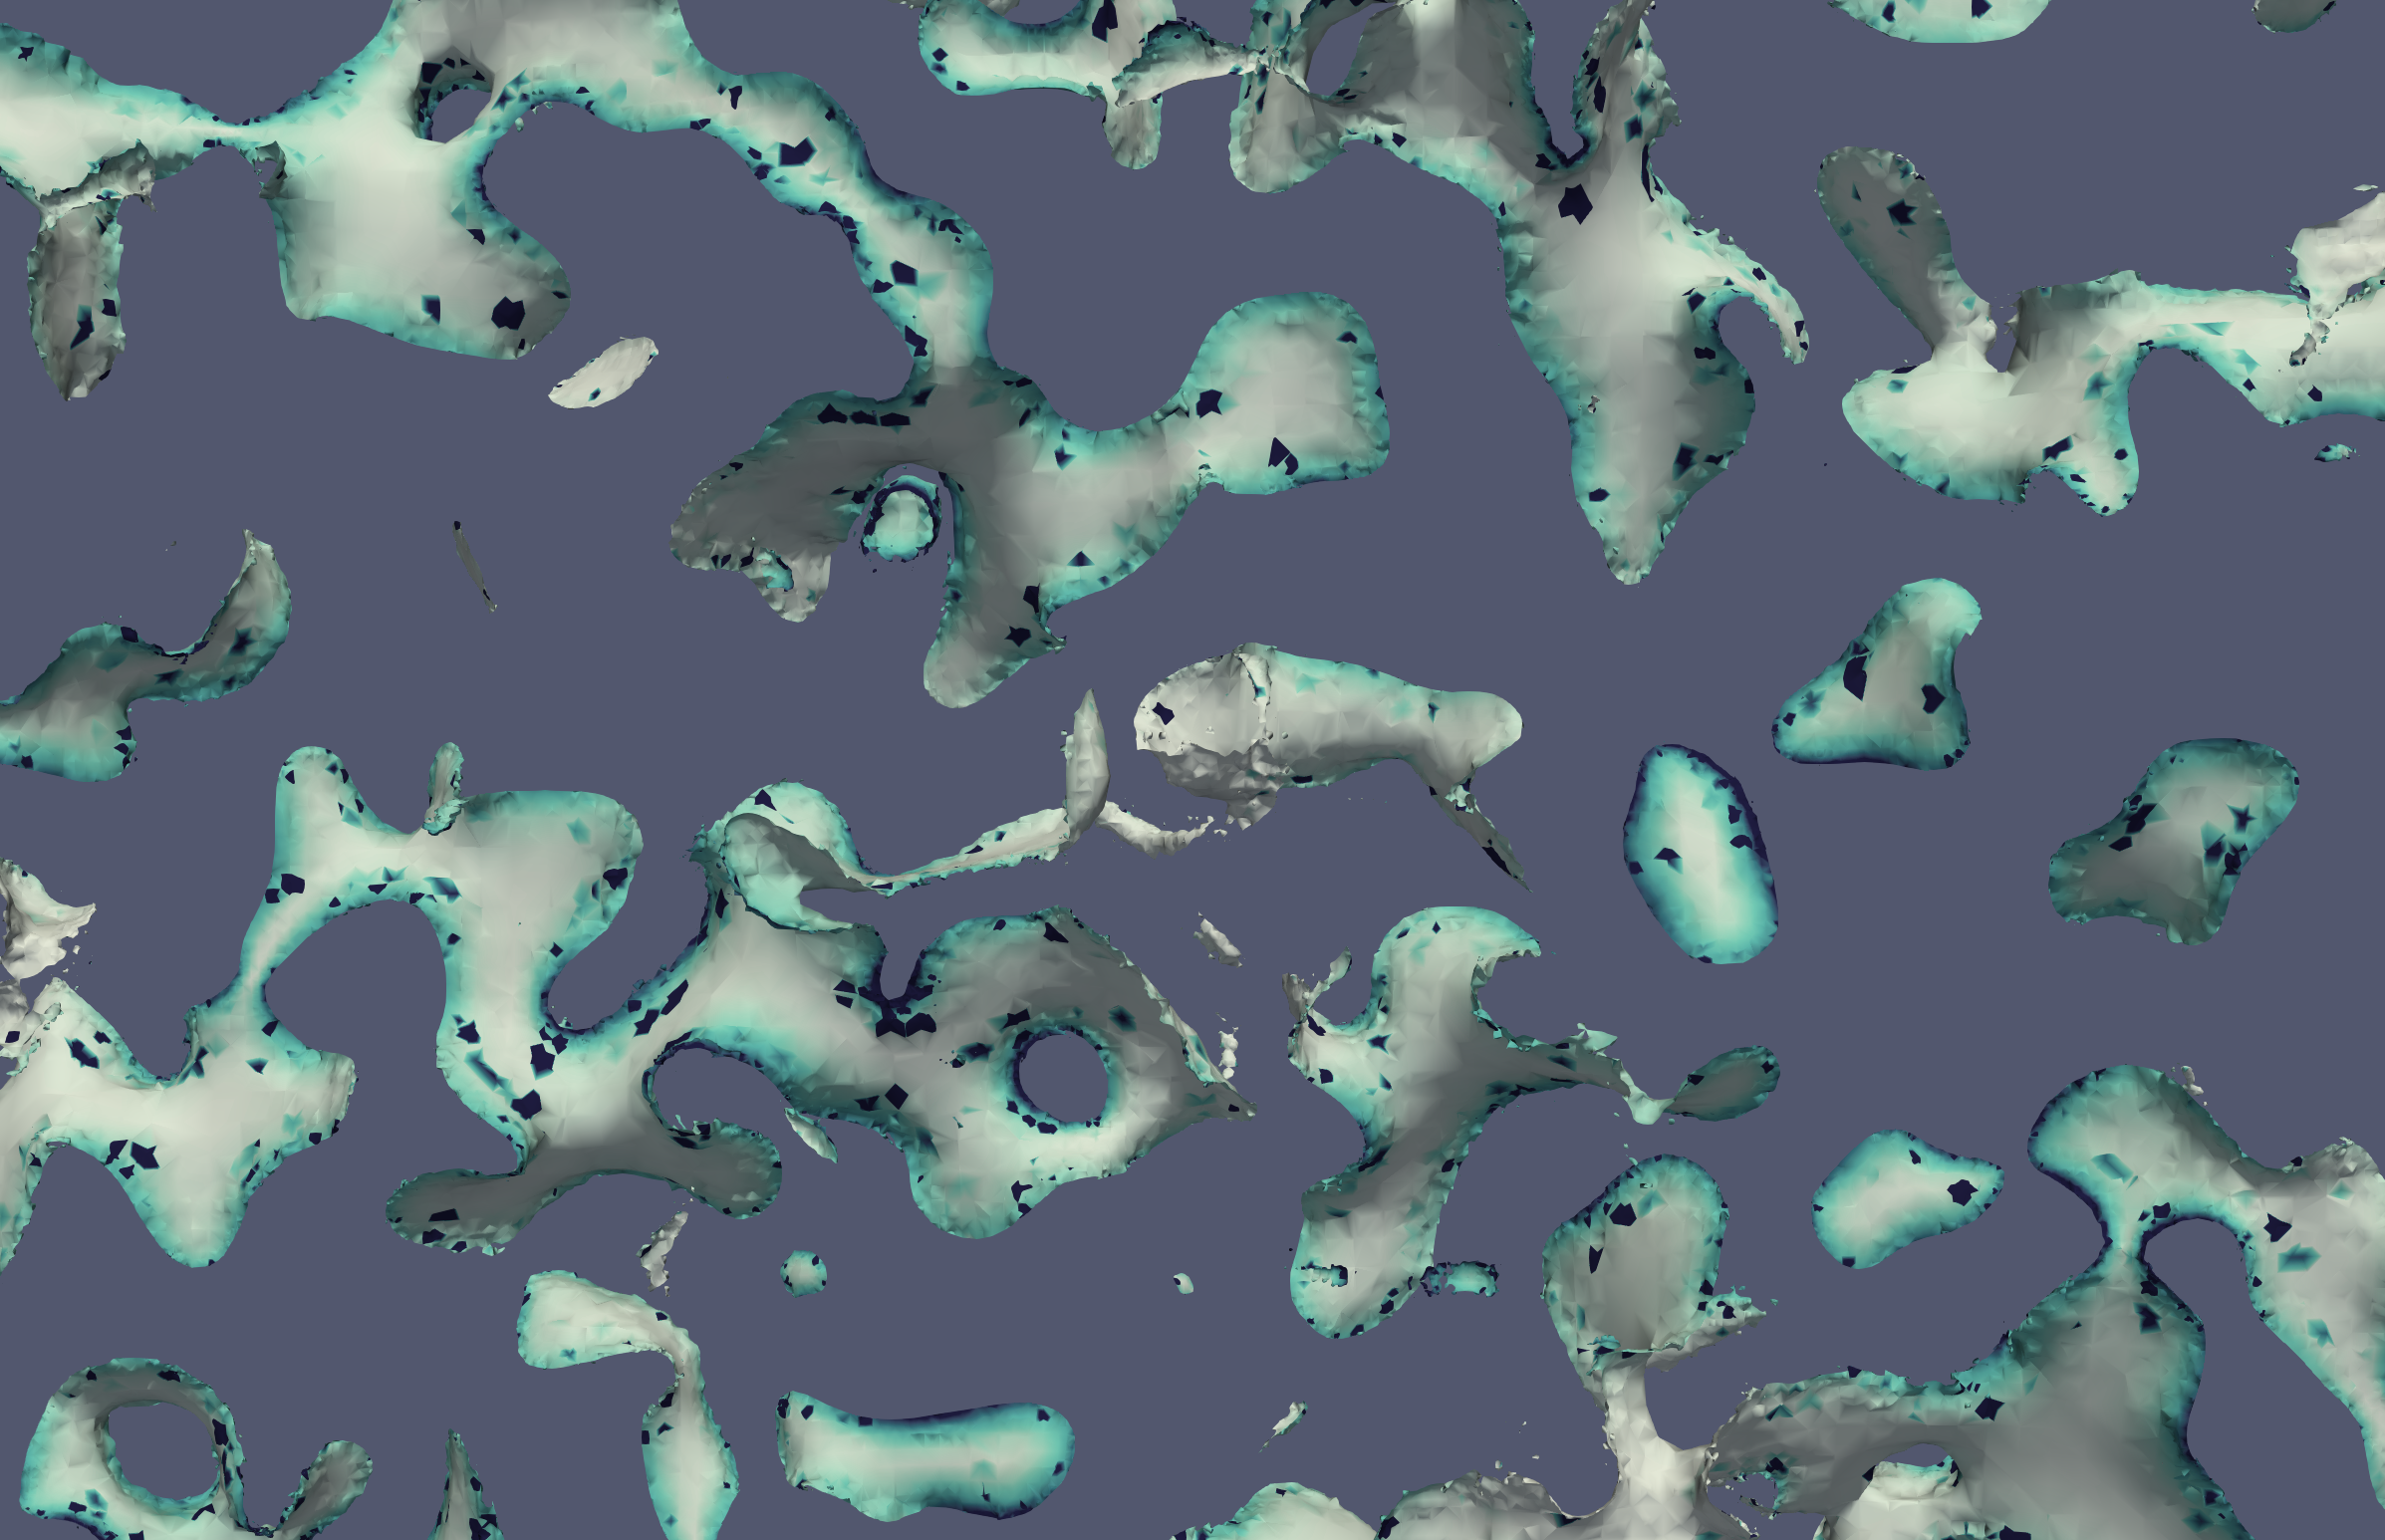
\includegraphics[height=8cm]{figures/nummeric_noise.png}
\caption{A visualization of the energy dissipation tensor $|\mathbf{\nabla}\otimes \mathbf{u}|$ on a iso-pressure surface of PM1, indicating the numerical issues that are accompanied by gradients of the velocity vector.}
\label{fig:numerical noise}
\end{figure}



\section{Histograms of $\mathcal{R}$ and $L_{\rm{eff}}$}

In Fig. S4 we plotted the histograms of  $\mathcal{R}_{\rm{meas}}$, $\mathcal{R}_{\rm{HP}}$, $\mathcal{R}_{\rm{m}}(f_2)$ and in Fig. S5 we have
The plots include a Kernal Density Estimate (KDE) of the distributions. In Fig. S5 we have shown the histograms of $L_{\rm{eff}}$, all resembling a log-normal distribution. These distributions could potentially be used to build a statistical network with equivalent network topology, with each bond representing a pore with a stochastic resistance drawn from these distributions. 



\begin{figure}
\setfigurenum{S4} %%You can change number for each figure if you want, not required. "S" prepended automatically.
\noindent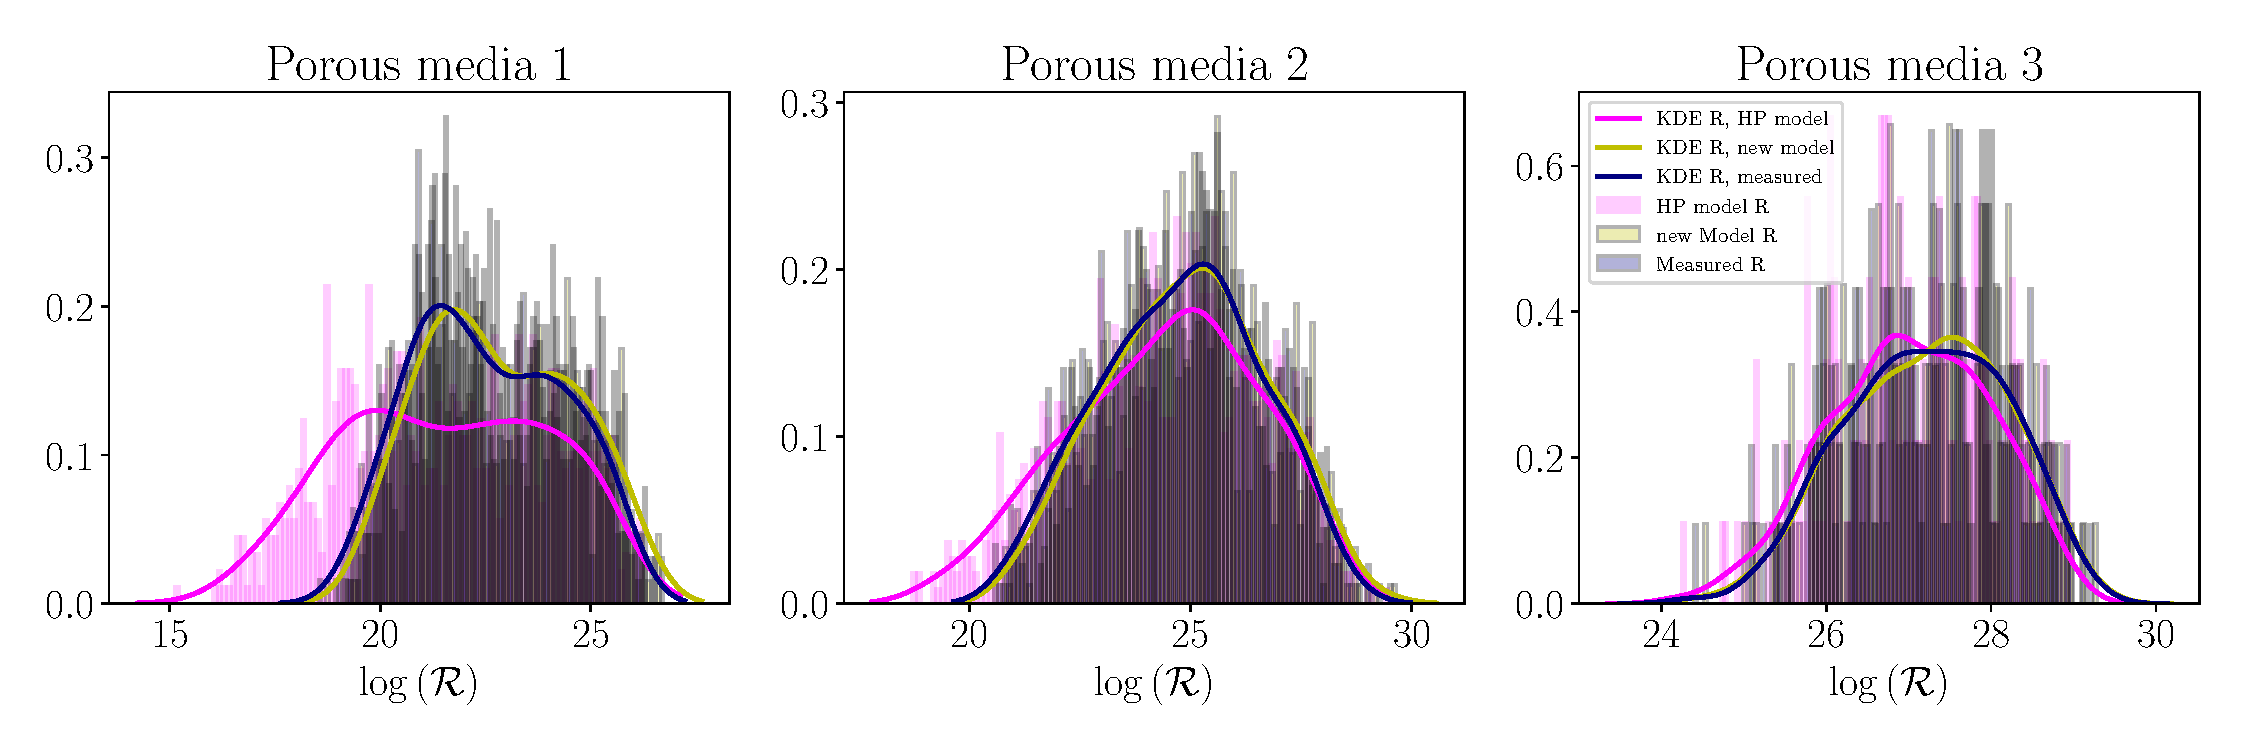
\includegraphics[width=15cm]{figures/hydraulic_resistance_integrated_histogram.pdf}
\caption{Histograms of the measured parameter space. }\label{Fig:Hist}
\end{figure}

\begin{figure}
\setfigurenum{S5} %%You can change number for each figure if you want, not required. "S" prepended automatically.
\noindent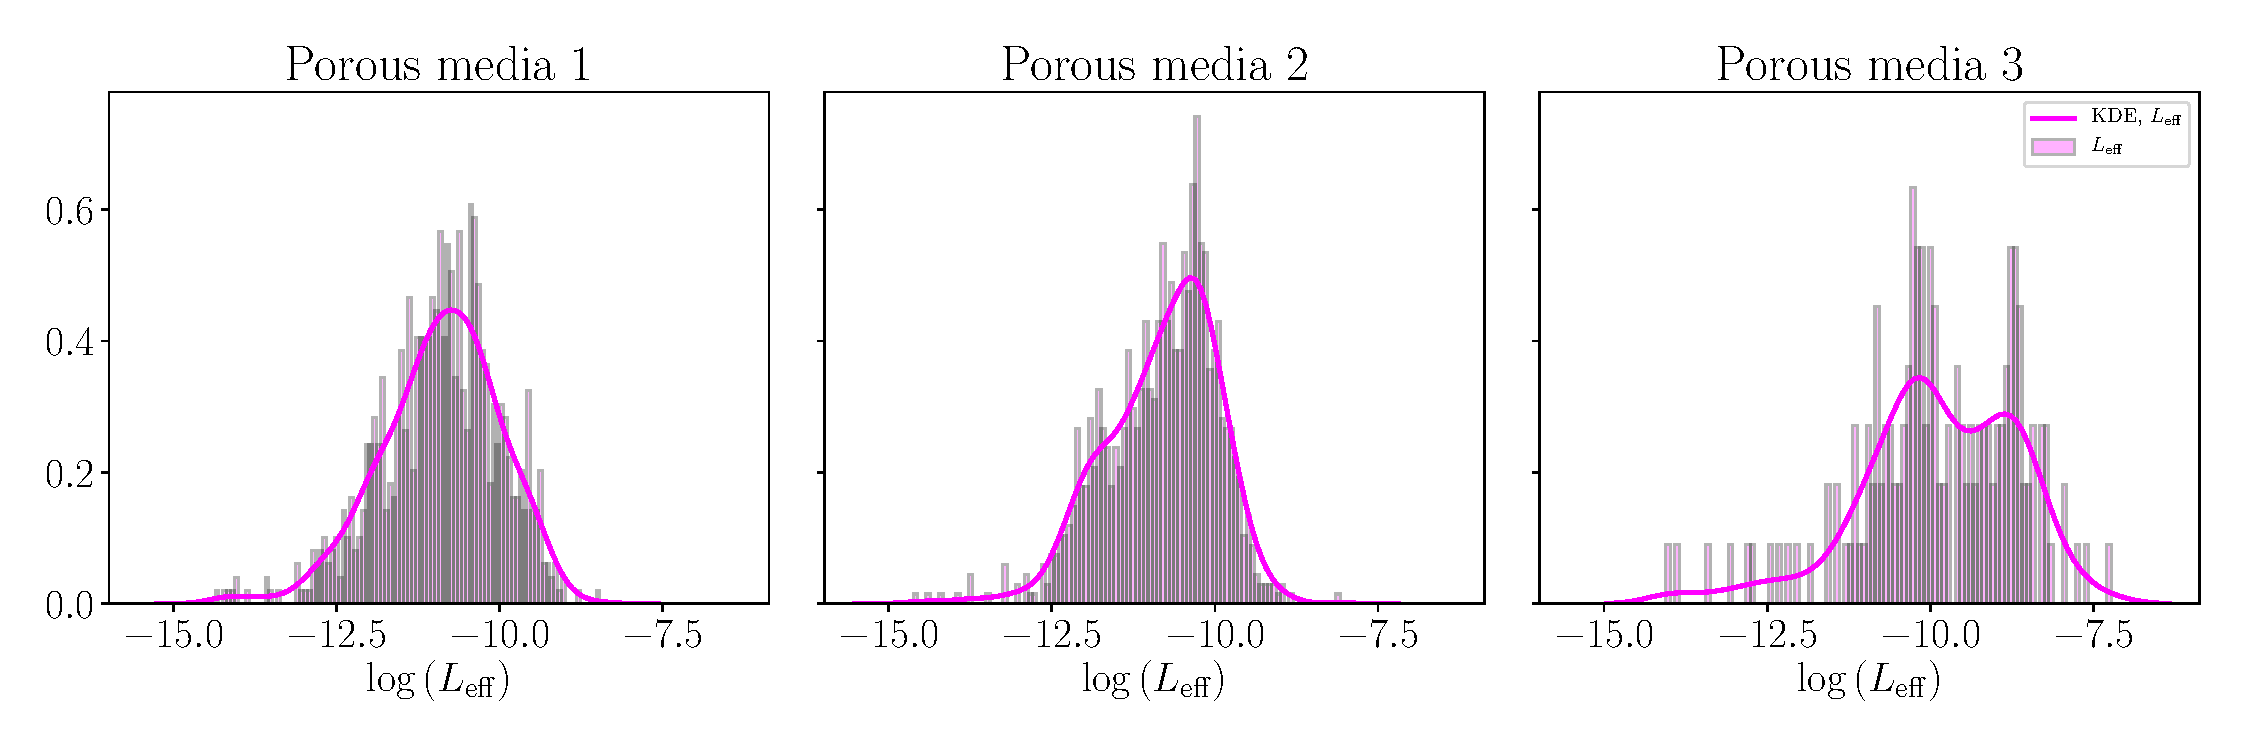
\includegraphics[width=15cm]{figures/Leff_integrated_histogram.pdf}
\caption{Histograms of the measured parameter space. }\label{Fig:Hist}
\end{figure}

\bibliography{library.bib}

% Copy/paste for multiples of each file type as needed.

% enter figures and tables below here: %%%%%%%
%
%
%
%
% EXAMPLE FIGURES
% ---------------
% If you get an error about an unknown bounding box, try specifying the width and height of the figure with the natwidth and natheight options.
% \begin{figure}
%\setfigurenum{S1} %%You can change number for each figure if you want, not required. "S" prepended automatically.
% \noindent\includegraphics[natwidth=800px,natheight=600px]{samplefigure.eps}
%\caption{caption}
%\label{epsfiguresample}
%\end{figure}
%
%
% Giving latex a width will help it to scale the figure properly. A simple trick is to use \textwidth. Try this if large figures run off the side of the page.
% \begin{figure}
% \noindent\includegraphics[width=\textwidth]{anothersample.png}
%\caption{caption}
%\label{pngfiguresample}
%\end{figure}
%
%
%\begin{figure}
%\noindent\includegraphics[width=\textwidth]{athirdsample.pdf}
%\caption{A pdf test figure}
%\label{pdffiguresample}
%\end{figure}
%
% PDFLatex does not seem to be able to process EPS figures. You may want to try the epstopdf package.
%
%
% ---------------
% EXAMPLE TABLE
%
%\begin{table}
%\settablenum{S1} %%Change number for each table
%\caption{Time of the Transition Between Phase 1 and Phase 2\tablenotemark{a}}
%\centering
%\begin{tabular}{l c}
%\hline
% Run  & Time (min)  \\
%\hline
%  $l1$  & 260   \\
%  $l2$  & 300   \\
%  $l3$  & 340   \\
%  $h1$  & 270   \\
%  $h2$  & 250   \\
%  $h3$  & 380   \\
%  $r1$  & 370   \\
%  $r2$  & 390   \\
%\hline
%\end{tabular}
%\tablenotetext{a}{Footnote text here.}
%\end{table}
% ---------------
%
% EXAMPLE LARGE TABLE (UPLOADED SEPARATELY)
%\begin{table}
%\settablenum{S1} %%Change number for each table
%\caption{Time of the Transition Between Phase 1 and Phase 2\tablenotemark{a}}
%\end{table}


\end{document}

%%%%%%%%%%%%%%%%%%%%%%%%%%%%%%%%%%%%%%%%%%%%%%%%%%%%%%%%%%%%%%%

More Information and Advice:

%% ------------------------------------------------------------------------ %%
%
%  SECTION HEADS
%
%% ------------------------------------------------------------------------ %%

% Capitalize the first letter of each word (except for
% prepositions, conjunctions, and articles that are
% three or fewer letters).

% AGU follows standard outline style; therefore, there cannot be a section 1 without
% a section 2, or a section 2.3.1 without a section 2.3.2.
% Please make sure your section numbers are balanced.
% ---------------
% Level 1 head
%
% Use the \section{} command to identify level 1 heads;
% type the appropriate head wording between the curly
% brackets, as shown below.
%
%An example:
%\section{Level 1 Head: Introduction}
%
% ---------------
% Level 2 head
%
% Use the \subsection{} command to identify level 2 heads.
%An example:
%\subsection{Level 2 Head}
%
% ---------------
% Level 3 head
%
% Use the \subsubsection{} command to identify level 3 heads
%An example:
%\subsubsection{Level 3 Head}
%
%---------------
% Level 4 head
%
% Use the \subsubsubsection{} command to identify level 3 heads
% An example:
%\subsubsubsection{Level 4 Head} An example.
%
%% ------------------------------------------------------------------------ %%
%
%  IN-TEXT LISTS
%
%% ------------------------------------------------------------------------ %%
%
% Do not use bulleted lists; enumerated lists are okay.
% \begin{enumerate}
% \item
% \item
% \item
% \end{enumerate}
%
%% ------------------------------------------------------------------------ %%
%
%  EQUATIONS
%
%% ------------------------------------------------------------------------ %%

% Single-line equations are centered.
% Equation arrays will appear left-aligned.

Math coded inside display math mode \[ ...\]
 will not be numbered, e.g.,:
 \[ x^2=y^2 + z^2\]

 Math coded inside \begin{equation} and \end{equation} will
 be automatically numbered, e.g.,:
 \begin{equation}
 x^2=y^2 + z^2
 \end{equation}

% IF YOU HAVE MULTI-LINE EQUATIONS, PLEASE
% BREAK THE EQUATIONS INTO TWO OR MORE LINES
% OF SINGLE COLUMN WIDTH (20 pc, 8.3 cm)
% using double backslashes (\\).

% To create multiline equations, use the
% \begin{eqnarray} and \end{eqnarray} environment
% as demonstrated below.
\begin{eqnarray}
  x_{1} & = & (x - x_{0}) \cos \Theta \nonumber \\
        && + (y - y_{0}) \sin \Theta  \nonumber \\
  y_{1} & = & -(x - x_{0}) \sin \Theta \nonumber \\
        && + (y - y_{0}) \cos \Theta.
\end{eqnarray}

%If you don't want an equation number, use the star form:
%\begin{eqnarray*}...\end{eqnarray*}

% Break each line at a sign of operation
% (+, -, etc.) if possible, with the sign of operation
% on the new line.

% Indent second and subsequent lines to align with
% the first character following the equal sign on the
% first line.

% Use an \hspace{} command to insert horizontal space
% into your equation if necessary. Place an appropriate
% unit of measure between the curly braces, e.g.
% \hspace{1in}; you may have to experiment to achieve
% the correct amount of space.


%% ------------------------------------------------------------------------ %%
%
%  EQUATION NUMBERING: COUNTER
%
%% ------------------------------------------------------------------------ %%

% You may change equation numbering by resetting
% the equation counter or by explicitly numbering
% an equation.

% To explicitly number an equation, type \eqnum{}
% (with the desired number between the brackets)
% after the \begin{equation} or \begin{eqnarray}
% command.  The \eqnum{} command will affect only
% the equation it appears with; LaTeX will number
% any equations appearing later in the manuscript
% according to the equation counter.
%

% If you have a multiline equation that needs only
% one equation number, use a \nonumber command in
% front of the double backslashes (\\) as shown in
% the multiline equation above.

%% ------------------------------------------------------------------------ %%
%
%  SIDEWAYS FIGURE AND TABLE EXAMPLES
%
%% ------------------------------------------------------------------------ %%
%
% For tables and figures, add \usepackage{rotating} to the paper and add the rotating.sty file to the folder.
% AGU prefers the use of {sidewaystable} over {landscapetable} as it causes fewer problems.
%
% \begin{sidewaysfigure}
% \includegraphics[width=20pc]{samplefigure.eps}
% \caption{caption here}
% \label{label_here}
% \end{sidewaysfigure}
%
%
%
% \begin{sidewaystable}
% \caption{}
% \begin{tabular}
% Table layout here.
% \end{tabular}
% \end{sidewaystable}
%
%

